\documentclass[a4paper,12pt]{report}
\usepackage[slovak,english]{babel}
\usepackage[T1]{fontenc}             
\usepackage[utf8]{inputenc}    
\usepackage{amsmath}
\usepackage{amssymb,amsfonts,amscd}
\usepackage{array,hhline}
\usepackage{makeidx}
\usepackage{fancyhdr}
\usepackage{graphicx}
\usepackage{listings}
    %%\usepackage{titlepage}
    %%\usepackage{multicol}
\usepackage{eurosym}
\usepackage{url,mathptmx} 
\usepackage[pdftex,unicode,bookmarks=false]{hyperref}

\usepackage[version=0.96]{pgf}
\usepackage{tikz}
\usetikzlibrary{arrows,shapes,snakes,automata,backgrounds,petri}

\usepackage{dirtree}


\renewcommand{\baselinestretch}{1.5}  % pre zvascenie riadkovania

\addtolength{\oddsidemargin}{-.5cm}
\addtolength{\evensidemargin}{-2.9cm}   
\addtolength{\topmargin}{0cm}
\addtolength{\textheight}{0pt}
\addtolength{\textwidth}{2.cm}
\addtolength{\textheight}{2.cm}
\newlength{\verbcorr}
\setlength{\verbcorr}{0ex}


\begin{document}
\selectlanguage{slovak}


\pagestyle{empty}
\pagenumbering{arabic}

\begin{titlepage}
\phantom.

\bigskip

\begin{center}
{\sc\LARGE Žilinská Univerzita v Žiline}
\medskip

{\sc\Large Fakulta riadenia a informatiky}

\vfill\vfill\vfill\vfill

{\sc\LARGE Diplomová práca}

\medskip

{\large Študijný odbor: {\bf Informačné a riadiace systémy}}
\end{center}


\vfill\vfill\vfill\vfill


\phantom.\hfill
\begin{minipage}{10cm}
\begin{center}
{\large\bf Meno Priezvisko}

\medskip

{\large\bf NÁZOV DIPLOMOVEJ PRÁCE \\   
aj na 2 riadky}

\medskip

Vedúci: {\bf doc. RNDr. Štefan Peško, CSc.}

\medskip
 
\hfill
Reg.č. xxx/2008 
\hfill
Máj 2012
\hfill\phantom.
\end{center}
\end{minipage}
\hspace{1.7cm}\phantom.

\vspace{2.9cm}

\phantom.
\end{titlepage}


%--------------------------------------------------------------------------------------
%%% slovensky abstrakt

\begin{abstract}

\noindent
{\sc Priezvisko Meno:} {\em Názov diplomovej práce}
[Diplomová práca] 

\noindent
Žilinská Univerzita v~Žiline,  
Fakulta riadenia a informatiky,  
Katedra matematických metód.

\noindent  
Vedúci: doc. RNDr. Štefan Peško, CSc. 
 
\noindent  
Stupeň odbornej kvalifikácie:
Inžinier v~odbore .... Žilina. 

\noindent
FRI ŽU v~Žiline, 2012 --- ?? s.

\bigskip

Obsahom práce je...


\end{abstract}


%--------------------------------------------------------------------------------------
%%% anglicky abstrakt


\selectlanguage{english}
\begin{abstract}

\noindent
{\sc Priezvisko Meno:} {\em Name of the Diploma thesis}
[Diploma thesis] 

\noindent
University of Žilina,  
Faculty of Management Science and Informatics, 
Department of mathematical methods.
 
\noindent
Tutor:  Assoc. Prof. RNDr. Štefan Peško, CSc. 
 
\noindent
Qualification level:
Engineer in field ..... Žilina: 

\noindent
FRI ŽU v Žiline, 2009 --- ?? p.

\bigskip

The main idea of this ...

\end{abstract}
\selectlanguage{slovak}


%%%%%%%%%%%%%%%%%%%%%%%%%%%%%%%%%%%%%%%%%%%%%%%%%%%%%%%%%%%%%%%%%%%%%%%
\newpage

\centerline{\bf Prehlásenie}

\vspace{2em}

\noindent
Prehlasujem, že som túto prácu napísal samostatne a že som uviedol 
všetky použité pramene a literatúru, z~ktorých som čerpal. 

\vspace{2em}

\noindent
V~Žiline, dňa 15.5.2012
\hfill
Meno Priezvisko

		% Titulna strana, Abstrakt, Prehlasenie, Predhovor


\pagestyle{myheadings}

%%%%%%%%%%%%%%%%%% obsah

{\setlength{\parskip}{1pt plus 1pt}

\markboth{}{}

\tableofcontents
}

\markboth{}{}

\clearpage

%%%%%%%%%%%%%%%%%% obsah - koniec


%%%%%%%%%%%%%%%%%% kapitoly

\chapter*{Úvod}
\addcontentsline{toc}{chapter}{Úvod}

Nájsť v dnešnej dobe zariadenie, ktoré neobsahuje mikrokontrolér je vzácnosť. Ceny týchto jednoduchých
počítačov klesli tak prudko, že sa s nimi stretávame na každom kroku. Z mnohých aplikácii sú to napríklad : automobily, riedenie v priemysle, mp3 prehrávače, alebo mobilné telefóny. Výkon dnešných
mikrokontrolérov je už dostatočne veľký pre beh veľmi zložitých programov. Pre udržanie prehľadnosti riešenia, vysokej modularity a efektívneho využitia zdrojov je dobré zahrnúť do programového vybavenia operačný systém. 

Práca si kladie za cieľ predstaviť koncepciu a realizáciu operačného systému pre jednočipový mikropočítač. Z dostupných mikrokontrolérov bol ako primárna platforma zvolený STM32F100 s jadrom Cortex M3, výrobca ST Microelectronics. Pre budúce použitie a rozšíriteľnosť bol tento systém upravný tak aby bol prenositeľný na mikrokontrolér LM4F120 s jadrom Cortex M4, výrobca Texas Instruments. Operačný systém je napísany veľmi jednoducho, môže tak slúžiť ako ukážkový príklad pre prípadného záujemcu. Koncepcia systému je plne modulárna, najmä vďaka použitiu mikrokernela a umožňuje po prepísaní jadra portovať ho na mnohé iné architektúry. 

Celá práca vznikla využitím open source nástrojov v prostrední Ubuntu Linux a ukazuje tak možnosť robiť plnohodnotný vývoj vstavných systémov v alternatívnom prostredí.
		%  Úvod
\chapter{Popis jadra cortex M3}
\section{Úvod}


Prvé mikroprocesory úspešne napredovali vo zvyšovaní výkonu vďaka zvyšovaniu počtu inštrukcií a zvyšovaniu taktovacej frekvencie. V 80-tych rokoch sa však ukázalo, že to nie je najlepšia cesta - dekóder inštrukcií mikroprocesora bol so vzrastajúcim počtom inštrukcií čoraz zložitejší a nastávali aj problémy so zreťazením inštruckií, či predikciou skokov. Páni Steve Furber a Sophie Wilson \cite{root_arm} si po preštudovaní dostupných publikácií a dôkladnej analýze uvedomili silné možnosti architektúry RISC 1, ktorá ponúkala pozoruhodný výpočtový výkon len so 44000 tranzistormi a 31 inštrukciami. Kľúčovou myšlienkou bol fakt, že ani programátor, ani kompilátor nedokážu optimálne využiť komplexné sady inštrukcií. 

Ich práca a vznik firmy Acorn vydláždili cestu k architektúre ARM 1. Prvé ARM jadro malo troj stupňové zreťazenie - načítanie, dekódovanie a vykonanie inštrukcie bolo v idéalnom prípade vykonávané pre tri inštrukcie naraz, každá v inom štádiu. Problém predstavovali a do dnes predstavujú inštrukcie podmienených skokov. Redukovaním počtu inštrukcií a prístupom do pamäte len pomocou inštrukcií load store tento neduh veľmi dobre redukuje. Ďalším prínosom ARM 1 jadra bol veľký počet registrov (pôvodne 37), všetky sú rovnocenné a dokonca programový čítač je namapovaný k týmto registrom, čo opäť umožňuje znížiť počet inštrukcií. Túto techniku využíva aj jadro msp430 \cite{msp430_mcu} .

Netrvalo dlho a vývojári si osvojili výhody jadra ARM. Dnes je známych mnoho verzií. Pre ilustráciu sú to napríklad popuĺárne ARM7TDMI, ARM11, ARM Cortex M, ARM Cortex R a veľmi výkonná rada ARM Cortex A \cite{arm_list} . Séria jadier Cortex A je populárna najmä v aplikačnej oblasti : inteligentné telefóny, tablety, dvd a blue ray prehrávače. Dá sa očakávať ich postupné nasadenie v osobných počtačoch. Výhodou je najmä spotreba a cena, ktorú znižuje nadol silná konkurencia.

Práca je zameraná na jadro Cortex m3 a Cortex m4. Je to rada so širokým spektrom použitia, najmä pre priemyselné aplikácie, aplikácie s nízkou spotrebou a citlivé na cenu. Najlepším príkladom ich porovnania, z pohľadu inštrukčnej sady je nasledujúci obrázok.

\begin{figure}[ht]
\begin{center}
\begin{minipage}{1.1\linewidth}
\begin{center}
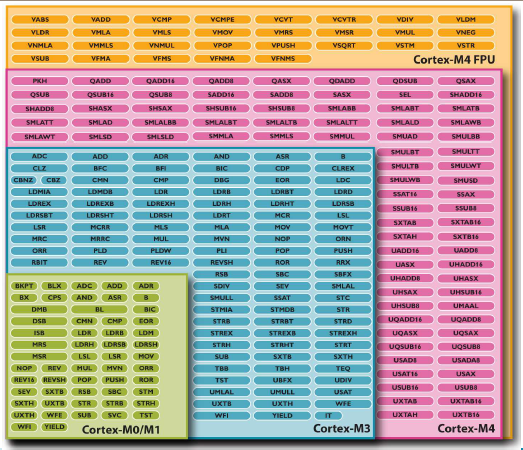
\includegraphics[width=.8\textwidth]{images/cm_instructions.png}
\caption{Porovnanie jadier Cortex Mx }
\label{obr1}
\end{center}
\end{minipage}
\end{center}
\end{figure}

Z obrázku je zrejmé, že jadrá sú navzájom kompatibilné, smerom k nižším modelom. Z konkrétnych typov mikrokontrolérov boli zvolené stm32f100 a lm4f120. Najmä pre ich bezproblémovú dostupnosť a cenu. Ako programátor pre stm32 bola použitá doska stm32 discovery kit a pre lm4f120 doska stellaris launchpad. Cena oboch dosiek je vzhľadom na možnosti použitia veľmi nízka (pod 15eur). S doskami je možné programovať aj mikrokontroléry v externej aplikácií, stačí počítač s USB rozhraním.

Pre samotné pochopenie a analýzu operačného systému je ale treba najprv rozobrať ich vnútornú, najmä registrovú štruktúru a princip funkcie radiča prerušení.

\section{Popis registrov}

Pre správnu funkciu mikroprocesora stačí minimum registrov : programový čítač, stavový register a register práve vykonávanej inštrukcie. Takto bolo navrhnuté jadro 68HC11 \cite{68HC11}. Obsahuje len dva univerzálne registre A, B, ukazovateľové registre X, Y a programový čítač spolu s ukazovateľom na zásobník. Snaha bola využiť dostupnú pamäť ako priestor na usutočňovanie všetkých operácií. Pre zvýšenie výpočtového výkonu, to však bola nesprávna cesta. Mikroprocesor musel takmer vždy vyberať operandy z pamäte a tieto operácie zaberú viac času, ako prístup do registrov. Jadro ARM preto zvolilo cestu vysokého počtu registrov. Problém nízkeho počtu registrov je aj v nemožnosti zreťazenia inštrukcií - inštrukcie je možné vykonávať paralelne len ak nie sú na sebe závislé (konflikt rovnakých registrov, alebo rovnaké adresy v pamäti).

Jadro ARM pre minimalizáciu počtu prístupov do pamäte využíva vysoký počet univerzálnych registrov. Registre R0 až R12 sú univerzálne použiteľné a dostupné pre aplikáciu. Register R13 je ukazovateľ zásobníka. Register R14 predstavuje tzv. Link register. Mikroprocesor doň ukladá návratovú adresu funkcie. Pri jednoúrovňových volaniach sa tak nemusí pristupovať na zásobník. Pre viacúrovňové volania sa už hodnota musí ukladať aj na zásobník, pričom posledne volaná funkcia má návratovú adresu vždy v LR registri. Programový čítač je prístupný ako register R15. Jadro je ďalej vybavené niekoľkými stavovými registrami, súhrnne označované ako xPSR. Tieto registre uchovávajú stav procesora a prerušení. Podrobnejší popis je možné nájsť v pekne spracovanej príručke Inside Cortex \cite{inside_cortex}

Inštrukčná sada ARM jadra plne využíva princíp load-store. Maximum operácií sa vykonáva medzi registrami. Nie je výnimkou použitie trojoperandových inštrukcií.  


\begin{figure}[ht]
\begin{center}
\begin{minipage}{1.1\linewidth}
\begin{center}
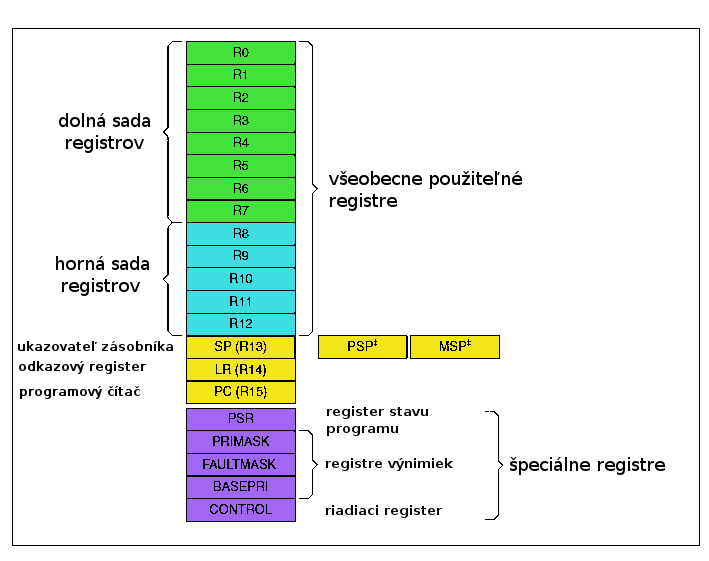
\includegraphics[width=.75\textwidth]{images/STM32F10xx_processor_core_registers.png}
\caption{Registre jadra Cortex M3 }
\label{obr2}
\end{center}
\end{minipage}
\end{center}
\end{figure}


\section{Jednotka NVIC}

Všetky mikrokontroléry s jadrom ARM Cortex sú vybavené pokročilou jednotkou správy prerušení. Jednotka NVIC je navrhnutá s ohľadom na minimalizáciu latencií prerušení. Taktiež zabezpečuje deterministickú obsluhu prerušení. Pre mikrokontrolér STM32F je k dispozícií 16 úrovní priorít prerušení.

Po hardvérovom generovaní prerušenia spustí NVIC sekvenciu niekoľkých krokov. Najprv sa dokončí práve vykonávaná inŠtrukcia. Následne sa pomocou mikrokódu uložia horné registre - nie je potrebný žiaden softvérovy zásah. Proces ukladania registrov trvá 12 hodinových cyklov. Následne sa spustí samotné vykonanie obsluhy prerušenia - užívateľská časť. Po ukončení vykonávania obsluhy sa opäť pomocou mikrokódu obnovia registre. Operácia obnovy taktiež trvá 12 cyklov.


\begin{figure}[ht]
\begin{center}
\begin{minipage}{1.1\linewidth}
\begin{center}
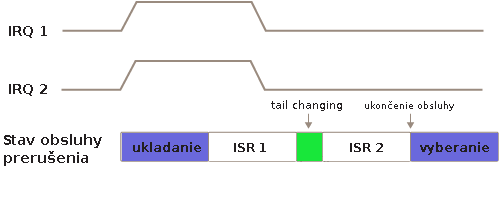
\includegraphics[width=.75\textwidth]{images/irq_sequence.png}
\caption{Sekvencia obsluhy prerušenia}
\label{obr2}
\end{center}
\end{minipage}
\end{center}
\end{figure}

Obrázok znázorňuje prioritný proces obsluhy dvoch prerušení. Prerušenie IRQ 1 má vyššiu prioritu. V krátkom okamihu nastanú požiadavky na obsluhu oboch prerušení. Jednotka NVIC uloží registre a spustí prvú obslužnú rutinu. Po jej ukončení sa vykoná tzv. tail changing - namiesto návratu do hlavnej slučky programu a opätovného ukladania registrov sa spustí obsluha druhého prerušenia. Táto operácia trvá len 6 strojových cyklov. Po dokončení obsluhy prerušenia sa obnovia registre a program pokračuje v hlavnej slučke.

Celkovo, sekvencia réžie trvá 30 strojových cyklov. Ak by nebola využitá možnosť tail changing, bolo by to 48 cyklov. Jednotka NVIC tak pomáha minimalizovať časové latencie a zjednodušiť návrh systému pracujúceho v reálnom čase.


\section{Tabuľka prerušení}

Prerušenie je reakcia na asynchronnú udalosť. Pôvodne bolo vyvinuté pre obsluhu pomalých periférií - procesor by bez prerušovacieho systému musel zbytočne čakať na dokončenie pomalej periférnej operácie. Vo svete programovania PC je možné sa stretnúť so softvérovými prerušeniami (int 10h, int 21h, int 80h). Názov je však zavádzajúci. V skutočnosti sa jedná o plne synchrónnu operáciu a je to volanie podprogramu uloženého na pevnej adrese.

Tabuľka prerušení jadra Cortex M3 má dve časti. V pamäti je však spojitá. Prvá časť sú vektory prerušení, spoločné pre všetky jadrá triedy Cortex M. Hneď za ňou sa nachádza druhá časť, ktorá obsahuje vektory závislé od použitých periférií. Nakoľko operačný systém má byť nezávislý od periférií, je z tohto pohľadu dôležitá len prvá časť. 

Treba poznamenať, že tabuľka musí byť uložená v sekcií isr\_vectors (nachádza sa obvykle na začiatku programovej pamäte). Prvá položka tabuľky je ukazovateľ na zásobník. Jadro podľa jej hodnoty nastavuje ukazovateľ zásobníka v RAM pamäti.


{\small
\begin{verbatim}
__attribute__ ((section(".isr_vector")))
void (* const g_pfnVectors[])(void) = {
					    // počiatočný stav zásobníka
    (void (*)(void))((unsigned long)pulStack + sizeof(pulStack)),
                                            
    ResetISR,                               // reset prerušenie
    NmiSR,                                  // NMI prerušenie
    FaultISR,                               // prerušenie kritického zlyhania
    ...
    SYS_TICK_INT,        	            // prerušenie systémového časovača
    ...
\end{verbatim}
}

Nasleduje položka \textbf{ResetISR}. To je vstupný bod do programu. Na tejto adrese začína mikrokontrolér vykonávať program. Táto funkcia obvykle predstavuje štartovaciu sekvenciu. Je však možné umiestniť sem ukazovateľ na funkciu main() a začať bez štartovacej sekvencie.

Z pohľadu stability systému je veľmi dobre využitá položka \textbf{FaultISR}. Toto prerušenie sa vyvolá pri vykonávaní nesprávnej alebo neoprávnenej inštrukcie. Odchytom tejto udalosti je možné emulovať napr. koprocesor v pohyblivej rádovej čiarke alebo využiť prerušenie na zotavenie systému z kritickej chyby. Ak sa nevyužijú tieto možnosti, je rozumné použiť ako obsluhu aspoň nekonečnú slučku.

{\small
\begin{verbatim}
static void FaultISR(void) {
    while(1)
    {
    }
}
\end{verbatim}
}

Ladiaci program to môže využiť a pomocou stavu zásobníka je možné dopracovať sa k pôvodu chyby.

Pre implementáciu preemptívneho multitaskingu je najdôležitejší vektor \textbf{SYS\_TICK\_INT}. Každé jadro Cortex M obsahuje systémový časovač. Ten je určený na jednoduché periodické vyvolávanie prerušenia. Vhodne napísanou rutinou obsluhy tejto udalosti je možné preemptívne prepínať kontext bežiacich procesov.

\section{Kontext procesora}

Pri implementacií multitaskingu je nevyhnutné poznať kontext použitého mikroprocesora. V najjednoduchšom prípade zahŕňa stav všetkých univerzálnych registrov. Rožšírením pojmu na kontext procesu je možné pridať aj ďalšie, nepovinné položky. Príkladom je zoznam zdrojov použitých procesom, alebo čitače prioritného plánovania. Nové mikrokontroléry automaticky ukladajú niektoré registre, pri začatí vykonávania rutiny obsluhy prerušenia. Nasledujúci obrázok ukazuje sériu operacií nad zásobníkom pre uloženie a obnovu kontextu \cite{context_switch}.

\begin{figure}[ht]
\begin{center}
\begin{minipage}{1.1\linewidth}
\begin{center}
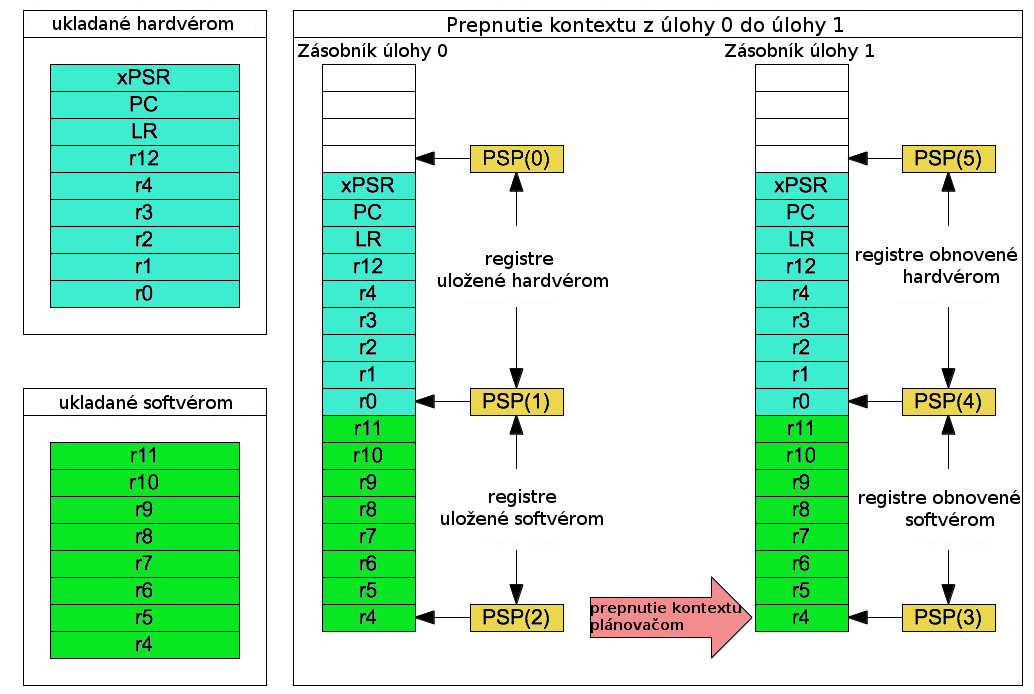
\includegraphics[width=.85\textwidth]{images/context_switch.png}
\caption{Prepnutie kontextu}
\label{obr2}
\end{center}
\end{minipage}
\end{center}
\end{figure}

Hardvér automaticky uloží registre R0..R5, R12, LR, PC a xPSR. V prípade jednoduchej obsluhy prerušenia to väčšinou postačuje a funkcia si vystačí s uvedenými registrami. V prípade prepnutia kontextu však nie je známe, či vlákna nevyužívajú aj zvyšné registre. Najmä pri rozsiahlejších funkciách kompilátor plne využije všetky registre. Nezostáva nič iné, ako uložiť všetky dostupné registre. Operácia je však veľmi rýchla a je realizovateľná jedinou inštrukciou :
{\small
\begin{verbatim}
__asm volatile("push {r4-r11}");
\end{verbatim}
}

Obnova kontextu je úplne analogická s ukladaním. Postupne sa vyberú registre, ktoré nie sú uložené hardvérom. Následne sa jadro informuje o tom, že sa vykonáva návrat z rutiny prerušenia, a že má vybrať aj zvyšné registre. Pokračujúca úloha bude teda opäť spustená bez zmeny registrov.
	%  Jadro CM3
\chapter{Analýza funkcií a architektúr operačných systémov}

Práca je zameraná na operačný systém pre vstavané systémy. Rozbor funkcionality operačných systémov bude preto zameraný najmä na túto oblasť. Mnoho rysov je spoločných pre každý operačný systém. Medzi výrazné odlišnosti od klasického systému pre osobný počítač, patria najmä veľmi obmedzená dostupná pamäť a pokročilý systém prerušení. Od toho je závislý pohľad na celkovú architektúru systému. V jednoduchých aplikáciach je možné použiť udalostne riadený systém. Zložitejšie vyžadujú prístup deterministického plánovača a fronty úloh. Druhým pohľadom je množina poskytovaných funkcií systému. Oba pohľady sú aplikačne závislé. Užívateľ by mal starostlivo zvážiť všetky potrebné požiadavky a podľa nich zvoliť koncepciu systému.

\section{Popis funkcií operačného systému}

Cieľom operačného systému je zabezpečiť kvalitné, stabilné a prehľadné rozhranie pre aplikačnú časť. Konkrétna množina funkcií je plne závislá od aplikácie. Medzi najčastejšie funkcie operačného systému patria:
\begin{itemize}
	\item Správa procesov a pamäte
	\item Medziprocesorová komunikácia
	\item Zabezpečenie synchronizácie operácií
	\item Všeobecne dostupné API rozhranie
\end{itemize}
Z ďalších funkcií je možné uviesť niekoľko špeciálnych a nie všeobecne typických pre každý operačný systém :
\begin{itemize}
	\item Ochrana pamäte
	\item Preemptívny multitasking
	\item Splnenie podmienok reálneho času
	\item Správa napájania
	\item Užívateľské rozhranie (textové alebo grafické)
\end{itemize}

Pre osobné počítače je v poslednej dobe typické najmä pokročilé užívateľské rozhranie. Z bežne dostupných sú to XFCE, KDE, Gnome a Unity
 \cite{linux_gui}. V ich prípade je v popredí častá interakcia s užívateľom systému. Preto je veľká pozornosť venovaná práve tejto časti.


V prípade vstavaných systémov je snaha vývojárov vytvoriť stabilný systém, kde nebude treba takmer žiaden dodatočný zásah zo strany programátora alebo užívateľa (s výnimkou upgradu). Typickým príkladom je mp3 prehrávač. Jeho užívateľské rozhranie sa rozhodne nemôže rovnať s rozhraním pre osobný počítač. V rámci možností hardvéru a najmä ceny, však poskytuje užívateľovi všetky potrebné funkcie. 

Príkladom systému, ktorý nedisponuje užívateľským rozhraním, sú ethernetové prepínače. Jednoduchšie prepínače realizujú posielanie rámcov uložením do medzipamäte. Po prijatí celého rámca a vyhodnotení adresy, sa rámec pošle ďalej. Toto všetko nevyžaduje žiadnu kontrolu od užívateľa.

Takmer nevyhnutnou súčasťou systému je medziprocesorová komunikácia. Najjednoduhšou formou je zdieľaná pamäť. Od nej je možné odvodiť ďalšie, pokročilejšie formy, najmä systém správ. V prípade viacúlohového systému, treba zabezpečiť vyhradený prístup do pamäte, čo predstavuje ďalšiu funkcionalitu systému - mutexy a semafóry. Táto množina funkcií vytvára základný balík pre pokročilú prácu so systémom.



\subsection{Synchronizácia úloh}

Každý viacúlohový operačný systém sa stretne s problémom synchronizácie dvoch a viacerých úloh. Táto situácia nastáva, ak aspoň dve vlákna požadujú vyhradený prístup k prostriedku. Tým môže byť napr. periférna operácia. Je potrebné preto zabezpečiť, aby druhé vlákno dostalo prístup k prostriedku až keď prvé ukončilo prácu s týmto zdrojom. Situáciu využitím jednoduchého mutexu modeluje nasledujúca Petriho sieť \cite{operacni_systemi}.

\begin{figure}[ht]
\begin{center}
\begin{minipage}{1.1\linewidth}
\begin{center}

\begin{tikzpicture}[node distance=1.3cm,>=stealth',bend angle=45]

  \tikzstyle{place}=[circle,thick,draw=blue!75,fill=blue!20,minimum size=6mm]
  \tikzstyle{red place}=[place,draw=red!75,fill=red!20]
  \tikzstyle{transition}=[rectangle,thick,draw=black!75,
  			  fill=black!20,minimum size=4mm]

  \tikzstyle{every label}=[red]
  \tikzstyle{language}=[Slovak]
  \begin{scope}
    % First net
     \node at (0,0) [place, tokens=1] (p1)  [label=above:{vlákno 1}]           {};
     \node at (0,-3) [place] (ks1) [label=left:$KS1$]                      {};
     \node at (0,-6) [place] (p2)                  {};


     \node at (4,0) [place, tokens=1] (q1)   [label=above:{vlákno 2}]               {};
     \node at (4,-3) [place] (ks2) [label=right:$KS2$]                      {};
     \node at (4,-6) [place] (q2)                  {};

     \node at (2,-3) [place, tokens=1] (sm) [label=above:$mutex$]                      {};


    \node at (0,-1.5)[transition] (e2) [label=left:{vstup}]  {}
      edge [pre]                (p1)
      edge [pre,bend left]      (sm)
      edge [post]               (ks1);


    \node at (0,-4.5)[transition] (e3) [label=left:{výstup}] {}
      edge [pre          ]      (ks1)
      edge [post,bend right]    (sm) 
      edge [post]               (p2);


    \node at (4,-1.5)[transition] (f2) [label=right:{vstup}]  {}
      edge [pre]                (q1)
      edge [pre,bend right]      (sm)
      edge [post]               (ks2);


    \node at (4,-4.5)[transition] (f3) [label=right:{výstup}] {}
      edge [pre          ]      (ks2)
      edge [post,bend left]    (sm) 
      edge [post]               (q2);

 \end{scope}  



  \begin{pgfonlayer}{background}
    \filldraw [line width=4mm,join=round,black!10]
      (p1.north  -| ks1.east)  rectangle (p1.south  -| ks1.west) ;
  \end{pgfonlayer}
\end{tikzpicture}


\caption {Synchronizácia procesov pomocou mutexu}
\label{obr1}
\end{center}
\end{minipage}
\end{center}
\end{figure}

Znázornené sú dve vlákna. Každé má svoju kritickú sekciu CSn. Vďaka použitiu mutexu môže vstúpiť do kritickej sekcie práve jedno vlákno. 
Označenie mutex je typické pre tzv. binárny semafór. Používajú sa všade tam, kde prostriedok môže byť pridelený len jednému procesu. V opačnom prípade je možné použiť klasický počítací semafór.

Treba poznamenať, že v prípade použitia jednoduchého mikrokontroléra je možné na vstup a výstup z kritickej sekcie použiť zakázanie, resp. povolenie prerušenia. Čas kedy je prerušenie zakázané, však treba obmedziť na minimum, aby nedošlo k narušeniu podmienok reálneho času a žiadostí na obsluhu prerušení.



\newpage
Ďalším typickým problémom synchronizácie, je riešenie problému čitateľov a zapisovateľa. Niekoľko vlákien číta dáta zo spoločnej pamäte. Čítanie je nedeštruktívne, preto môže k tejto zdieľanej oblasti pristupovať viac vlákien súčasne. Úloha zapisovateľa je do spoločnej pamäte zapísať dáta. Požaduje sa vyhradený prístup - zápis musí prebehnúť atomicky. Počas zápisu nemá žiaden z čitateľov prístup k pamäti. Situáciu je opäť možné modelovať Petriho sieťou.

\begin{figure}[ht]
\begin{center}
\begin{minipage}{1.1\linewidth}
\begin{center}

\begin{tikzpicture}[node distance=1.3cm,>=stealth',bend angle=45,auto]

  \tikzstyle{place}=[circle,thick,draw=blue!75,fill=blue!20,minimum size=6mm]
  \tikzstyle{red place}=[place,draw=red!75,fill=red!20]
  \tikzstyle{transition}=[rectangle,thick,draw=black!75,
  			  fill=black!20,minimum size=4mm]

  \tikzstyle{every label}=[red]

  \begin{scope}
    % First net
     \node at (0,0) [place, tokens=1] (p1)  [label=above:{vlákno R1}]           {};
     \node at (0,-3) [place] (ks1) [label=left:{čítanie}]                      {};
     \node at (0,-6) [place] (p2)                  {};


     \node at (3,0) [place, tokens=1] (q1)   [label=above:{vlákno R2}]               {};
     \node at (3,-3) [place] (ks2) [label=right:{čítanie}]                      {};
     \node at (3,-6) [place] (q2)                  {};

     \node at (10,0) [place, tokens=1] (r1)   [label=above:{vlákno W}]               {};
     \node at (10,-3) [place] (ks3) [label=right:{zápis}]                      {};
     \node at (10,-6) [place] (r2)                  {};

     \node at (8,-3) [place, tokens=2] (sm) [label=left:{semafor}]                      {};


    \node at (0,-1.5)[transition] (e2) [label=left:{vstup}]  {}
      edge [pre]                (p1)
      edge [pre,bend left]      (sm)
      edge [post]               (ks1);


    \node at (0,-4.5)[transition] (e3) [label=left:{výstup}] {}
      edge [pre          ]      (ks1)
      edge [post,bend right]    (sm) 
      edge [post]               (p2);


    \node at (3,-1.5)[transition] (f2) [label=right:{vstup}]  {}
      edge [pre]                (q1)
      edge [pre,bend left]      (sm)
      edge [post]               (ks2);


    \node at (3,-4.5)[transition] (f3) [label=right:{výstup}] {}
      edge [pre          ]      (ks2)
      edge [post,bend right]    (sm) 
      edge [post]               (q2);



    \node at (10,-1.5)[transition] (g2) [label=right:{vstup}]  {}
      edge [pre]                (r1)
      edge [pre,bend right]      (sm) [label=left:$2$]
      edge [post]               (ks3);


    \node at (10,-4.5)[transition] (g3) [label=right:{výstup}] {}
      edge [pre          ]      (ks3)
      edge [post,bend left]    (sm)  [label=left:$2$]
      edge [post]               (r2);

 \end{scope}  



  \begin{pgfonlayer}{background}
    \filldraw [line width=4mm,join=round,black!10]
      (p1.north  -| ks1.east)  rectangle (p1.south  -| ks1.west) ;
  \end{pgfonlayer}
\end{tikzpicture}


\caption {Problém čitateľov a zapisovateľa}
\label{obr1}
\end{center}
\end{minipage}
\end{center}
\end{figure}

Čitateľmi sú vlákna R1 a R2. Vždy pri požiadavke na čítanie odoberie čitateľ práve jeden token - druhý ostáva voľný pre druhé vlákno. Zapisovateľ však pri požiadavke na zápis musí odobrať dva tokeny. Tak zabráni vstupu ľubovoľného z čitateľov do kritickej sekcie, prípadne aj ďalšiemu zapisovateľovi. Princíp riešenia je totiž možné rozšíriť na ľubovoľný počet zapisovateľov i čitateľov.
Z praktických aplikácií tohto problému je možné uviesť napr. databázové systémy alebo klient-server aplikácie. Princíp je použiteľný aj pri prúdovom spracovaní číslicového signálu, napr. s využitím viacjadrového mikroprocesora. Treba poznamenať, že uvedená Petriho sieť nie je najspravodlivejším riešením. Ak budú čitatelia neustále vyžadovať prístup k dátam, zapisovateľ nikdy nedostane možnosť vstúpiť do kritickej sekcie. Na riešenie tejto situácie je potrebné využiť pomocný synchronizačný prostriedok, prípadne správu, ktorá informuje čitateĺov o novo aktualizovaných dátach.


\newpage

\subsection{Posielanie správ}

Existuje niekoľko vzácnych prípadov, kedy sú vlákna natoľko nezávislé, že nemusia spolu komunikovať. Vo veľkej väčšine aplikácií je však medzivláknová komunikácia nevynutná. Pomáha najmä pri dekompozícií riešeného problému a jeho rozdeleniu medzi viacero vlákien. Poslanie správy možno modelovať na Petriho sieti :

\begin{figure}[ht]
\begin{center}
\begin{minipage}{1.1\linewidth}
\begin{center}

\begin{tikzpicture}[node distance=1.3cm,>=stealth',bend angle=45,auto]

  \tikzstyle{place}=[circle,thick,draw=blue!75,fill=blue!20,minimum size=6mm]
  \tikzstyle{red place}=[place,draw=red!75,fill=red!20]
  \tikzstyle{transition}=[rectangle,thick,draw=black!75,
  			  fill=black!20,minimum size=4mm]

  \tikzstyle{every label}=[red]

  \begin{scope}
    % First net
     \node at (0,0) [place, tokens=1] (p1)  [label=above:{vlákno 1}]           {};
     \node at (0,-3) [place] (ks1)                      {};
     \node at (0,-6) [place] (p2)                  {};


     \node at (4,0) [place, tokens=1] (q1)   [label=above:{vlákno 2}]               {};
     \node at (4,-3) [place] (ks2) [label=right:{príjem}]                      {};
     \node at (4,-6) [place] (q2)                  {};

     \node at (2,-3) [place, tokens=1] (sm) [label=below:{posielanie}]                      {};


    \node at (0,-1.5)[transition] (e2) [label=left:{poslanie správy}]  {}
      edge [pre]                (p1)
      edge [post]               (ks1);


    \node at (0,-4.5)[transition] (e3) [label=left:{hotovo}] {}
      edge [pre          ]      (ks1)
      edge [post,bend right]    (sm) 
      edge [post]               (p2);


    \node at (4,-1.5)[transition] (f2) [label=right:{prijatie správy}]  {}
      edge [pre]                (q1)
      edge [pre,bend right]      (sm)
      edge [post]               (ks2);


    \node at (4,-4.5)[transition] (f3) [label=right:{hotovo}] {}
      edge [pre          ]      (ks2)
      edge [post]               (q2);

 \end{scope}  



  \begin{pgfonlayer}{background}
    \filldraw [line width=4mm,join=round,black!10]
      (p1.north  -| ks1.east)  rectangle (p1.south  -| ks1.west) ;
  \end{pgfonlayer}
\end{tikzpicture}

\caption {Posielanie správ medzi procesmi}
\label{obr1}
\end{center}
\end{minipage}
\end{center}
\end{figure}


V tomto prípade je použité synchronné prijímanie správ. Vlákno 2 čaká kým nepríjme správu. Existujú situácie, kde je to nežiadúce. Vtedy vlákno podľa potreby kontroluje príznak prítomnosti správy. Operácia príjímania je v tom prípade neblokujúca.

\newpage
\section{Architektúra operačných systémov}

Pri analýze systému je dôležitý pohľad celkovej koncepcie riešenia. Patrí sem rozdelenie na jednotlivé moduly, ktoré bloky bežia v prostredí jadra a ako sú implementované služby systému. Z tohto hľadiska je možné operačné systémy rozdeliť na tri skupiny :
\begin{itemize}
	\item Monolytické jadro
	\item Hybridné jadro
	\item Mikro jadro
\end{itemize}


\begin{figure}[htbp]
\begin{center}
\begin{minipage}{1.1\linewidth}
\begin{center}
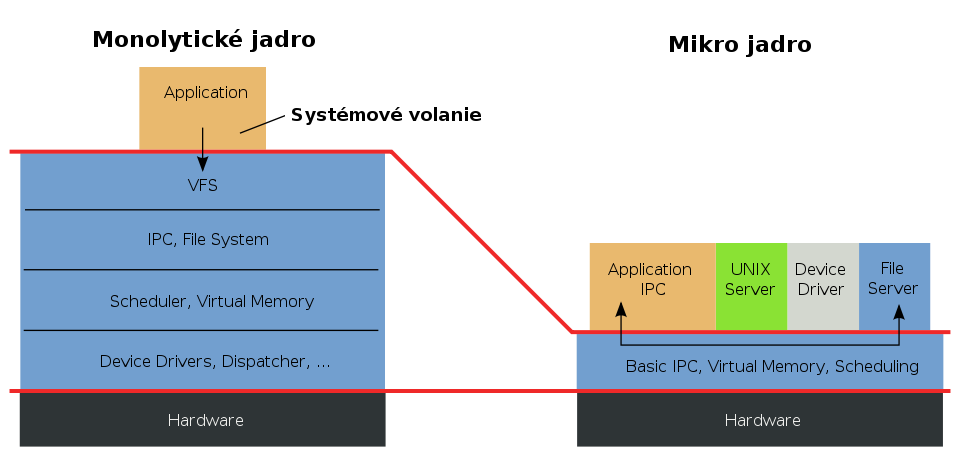
\includegraphics[width=0.8\textwidth]{images/os-structure_01.png}
\caption{Prehľad architektúr operačného systému}
\label{obr1}
\end{center}
\end{minipage}
\end{center}
\end{figure}


Nezávisle od aplikácie, je najdôležitejšou úlohou operačného systému správa procesov a prideľovanie procesorového času. Z pohľadu riešenia tejto časti (oblasť plánovača a prideľovania procesorového času) existujú systémy riadené striktne udalosťami, systémy spracovávajúce frontu úloh a samozrejme hybridné systémy. 

\begin{itemize}
	\item Udalostné systémy spúšťajú úlohy podľa výskytu udalostí - prerušenia alebo programovo generovaná udalosť. V princípe je to zovšeobecnenie systému prerušení pre akúkoľvek časť programu a nezávislosť od hardvéru. Táto koncepcia umožňuje realizovať systémy s krátkou dobou odozvy a výrazne šetrí pamäť.
	\item Systémy spracovávajúce frontu úloh poskytujú maximálnu robustnosť a flexibilitu. Typické sú pre ne pokročilé plánovacie algoritmy a prioritné prideľovanie zdrojov procesu.
	\item Hybridné riešenie kombinuje výhody oboch riešení.
\end{itemize}

\textbf{Monolitické jadro}
Tento model integruje všetky funkcie operačného systému do jedného bloku, tvoreného jadrom aj zvyškom systému. Volanie akejkoľvek funkcie systému je vždy realizované na úrovni jadra. Znižuje sa tak doba odozvy systému. Nevýhodou je narastajúca veľkosť jadra, aj čas strávený v priestore jadra. Mnohé moderné operačné sysemy (napr. Linux) riešia tento problém zavádzaním modulov do jadra až keď sú naozaj potrebné. Zvyšuje sa tak modularita systému. Typickými zástupcami sú Unix, Linux, FreeBSD, CP/M a MS-DOS. 

\textbf{Mikro jadro}
Jadro systému je minimalizované len na nevyhnutné funkcie - často len prepínanie úloh, správu pamäte a medziprocesorovú komunikáciu. Všetky ostatné služby sú riešené na aplikačnej úrovni. Často sa využíva model klient-server. Server je poskytovateľ služieb a beží ako samostatný proces. Klient požiada server o službu, komunikáciu sprostredkuje jadro. Systémy s týmto modelom sú veľmi robustné a spoľahlivé. Mnoho priemyselných aplikácií má práve túto architektúru. Nevýhodou môže byť dlhšia časová latencia na poskytnutie služby - systém ide vždy cestou : klient -> jadro -> server -> jadro -> klient. Typickými zástupcami sú QNX, Symbian OS, Phoenix-RTOS.

\textbf{Hybridné jadro}
Kombináciou výhod oboch prístupov vzniklo hybridné jadro. Časovo kritické a často volané služby bežia v prostedí jadra, ako v prípade monolytického systému. Služby nevyžadujúce rýchlu odozvu bežia ako jendotlivé servery. Príkladom je súborový systém, ktorý je relatívne pomalý voči ostatným službám. Najvýraznejším zástupcom v tejto kategórií je Windows NT.

\section{Klasifikácia systémov v závisloti na pricípe plánovania prepínania úloh}
\subsection{Udalostne riadené systémy}

Veľkú kategóriu operačných systémov vo vstavaných aplikáciach, tvoria systémy riadené udalosťami. Je to realizácia veľmi jednoduchej myšlienky : ak nie sú dáta, nie je čo robiť. Výrobcovia mikrokontrolérov si toto rýchlo uvedomili a vybavili mikrokontroléry pokročilým prerušovacím systémom. Táto koncepcia navyše umožňuje využiť režim zníženej spotreby - keď nie je udalosť, jadro procesora sa môže uspať.
Problematiku riadenia spotreby má veľmi dobre rozpracovanú firma Texas Instrumets so svojím 16 bitovým mikrokontrolérom s jadrom msp430 \cite {ti_msp430}.

Veľmi dobrou vlastnosťou tohto prístupu je spĺňanie podmienok reálneho času. To je veľmi dôležité hlavne v prípade číslicového spracovania signálu a v priemyselnom riadení. S využitím možností vnorených prerušení, je možné si poradiť aj s udalosťami vyskytujúcimi sa veľmi často (relatívne k času behu úloh - obsluhy prerušenia). Najlepšie situácu vystihne ukážka programu - blikanie led. Po reštarte treba inicializovať prerušenie od časovača a príslušný pin nastaviť ako výstup. Po povolení prerušení už nie je nutná účasť programu v hlavnej slučke - procesor je možné uspať a znížiť tak spotrebu. Vždy pri vyvolaní prerušovacej rutiny sa zmení stav na pine s led a vypne sa režim zníženej spotreby. Je vidieť, že v hlavnej slučke môže bežať ďalšia úloha.

{\small
\begin{verbatim}
int main()
{
 io_init();		  	  /*inicializácia hardvéru*/
 eint();			  /*globálne povolenie prerušení*/
 while (1)
  LPM0;				  /*vypnutie jadra procesora - zníženie spotreby*/
}

/*prerušenie časovača*/
interrupt(TIMER0_A0_VECTOR)  TIMER0_A0_ISR(void) 
{
 P1OUT^=0x01;	/*zmena stavu výstupu - led sa striedavo zapína a vypína*/
 LPM3_EXIT; 	/*znovu spustenie jadra po návrate z prerušenia*/
}
\end{verbatim}
}


Na pohľad vyzerá tento program veľmi jednoducho, ale má všetko potrebné pre reagovanie na jednoduchú udalosť. Veľký problém je hardvérová závislosť - prerušenia sú pevne zviazané s daným typom mikrokontroléra. Následne nie je možné program prenášať na iný mikrokontrolér. Problémom môže byť aj takmer nulová kontrola nad poradím a frekvenciou volaní prerušení. Riešením je vytvoriť programovú nadstavbu, ktorá zastreší systém prerušení aj systém volania udalostí. Princíp spočíva v minimalizácií programu v rutine obsluhy prerušenia - často stačí len nastavenie príznaku v globálnej premennej a okamžitý odchod z rutiny.

V anglickej literatúre sa tento princíp označuje ako event driven programming. Je to však pojem zaužívaný skôr pre programovanie osobných počítačov. Najčastejšie je tento princíp využívaný v spojení s grafickým rozhraním - kliknutie na tlačítko vyvolá udalosť OnClick. Operačný systém ju zachytí a pošle hlavnej slučke aplikácie. Samozrejmosťou je možnosť definovať vlastné udalosti. Treba poznamenať, že nad takouto správou udalostí beži pokročilý operačný systém. Možnosti realizovať to na mikrokontroléri bez preemptívneho multitaskingu však nič nebráni. 
V hlavnej slučke sa najprv overí fronta udalostí (zaslané prerušeniami alebo predošlými úlohami). Následne sa postupne vyberú a podľa adresy doručenia sa predávajú volaným úloham, napr. formou parametra funkcie.

Tento trend programovania je možné čoraz viac sledovať v mobilných zariadeniach \cite{android_event}. Aplikácia tak zbytočne nevyťažuje mikroprocesor a predlžuje sa životnosť batérie.

Priblíženie tohto populárneho spôsobu programovania na mikrokontroléroch, využila firma Quantum Leaps so svojim frameworkom QP \cite{qp_project}. Je to systém funkcií pre mikrokontroléry so veľmi odmedzenou kapacitou pamäťe. Projekt je založený na dekompozicií úlohy na stavové automaty. V hlavnej slučke programu sú v cykle spúšťané jednotlivé aktívne objekty. Existuje aj varianta pre populárnu vývojovú dosku Arduino. Projekt je uvoľnený ako Open Source pod GNU/GPL licenciou. V prípade problémov s touto licenciou (komerčná firma s inými požiadavkami), je možné vyjednať aj inú formu licencie.

Základným kameňom tohto projektu sú aktívne objekty. Výkonná časť algoritmu je realizovaná stavovým automatom. A objekty si medzi sebou vymieňajú dáta pomocou parametrov.

V nasledujúcej ukážke, je znázornený princíp objektov Qp. Úloha riešila problém obedujúcich filozofov. Jednotlivé časti problému boli rozdelené na niekoľko automatov (jednotlivé static QState Philo funkcie). Každá funkcia môže v sebe realizovať ďalší automat (podautomat, celkom nezávislý alebo jeden spoločný pre celý objekt).

{\small
\begin{verbatim}
typedef struct PhiloTag {
    QActive super;
} Philo;

static QState Philo_initial (Philo *me);
static QState Philo_thinking(Philo *me);
static QState Philo_hungry  (Philo *me);
static QState Philo_eating  (Philo *me);
\end{verbatim}
}

Vďaka princípu automatu môže zdanlivo paralelne bežať mnoho Qp objektov. Posielanie udalostí potom realizujú jednotlivé objekty. Systém Qp je tak vhodný pre riadenie procesov, nízkoenergetické aplikácie a mikrokontroléry s malým množstvom pamäte. Vďaka prehľadnému riešeniu rozdelením na objekty, umožňuje udržať prehľadnosť projektu a veľmi dobrú udržateľnosť produktu. K dispozícií je aj grafický nástroj na tvorbu systému.

Celkový pohľad na začlenenie Qp objektov v mikrokontroléri, znázorńuje nasledujúci obrázok. Je zrejmé, že systém Qp môže bežať pod kernelom iného operačného systému a tvoriť tak akýsi podsystém. V tom prípade sa však už zvýši doba odozvy, uplatnenie nájde aj v tejto podobe, napr. GUI pre riadenie dotykového displeja.

\subsection{Systémy s frontou úloh}

Veľkú skupinu operačných systémov tvorí klasický prístup k úlohovému spracovaniu. Je to najstaršia myšlienka využívaná už prvých zárodkoch operačných systémov. Tie jednoducho zoradili do fronty zoznam úloh a postupne ich spustili. Preempcia vtedy neexistovala, a tak úloha musela bez chyby zbehnúť, prípadne niekedy počas vykonávania predať riadenie opäť operačnému systému. Vznikali rôzne algoritmy ako zoradiť úlohy vo fronte, aby úlohy boli dokončené čo najoptimálnejšie - z hľadiska využitia procesora, aj z hľadiska spokojnosti užívateľa.
V navigačnom počítači Apolla bola použitá veľmi pokroková metóda plánovania - prioritné plánovanie. Je zrejmé, že systém navigácie lode spadá do kategórie tzv. mission critical systems. Preto boli úlohy so životne dôležitou funkciou vždy na začiatku fronty. Ak zostal po ich splnení procesorový čas, prešlo sa na spracovanie menej dôležitých úloh (chyba 1202 pri pristávaní Apolla 11). Všetky procesy ohľadom navigácie a stability lode však bolo potrebné plniť v prísne stanovených časových úsekoch. Ak nezostal čas na plnenie ďalšej menej dôležitej úlohy, úloha sa vôbec nezačala vykonávať - začal nový cyklus plánovača. Toto bol jeden z prvých systémov reálneho času a pravdepodobne prvý vstavaný systém na svete. Ešte dnes možno nájsť inšpiráciu vo vtedajšom prístupe k riešeniu. Problematike hardvéru aj softvéru počítača Apolla sa venuje \cite{apollo_agc}.

Nasledujúci program znázorňuje veľmi jednoduchý systém reálneho času, ktorý zabezpečuje periodické spúšťanie úloh.

{\small
\begin{verbatim}
/*ukazovateľ na funkciu a periodicita spúšťania*/
struct stCyclFunc {
		   u32 fFunc;
                   u32 bTimeStamp;
		  };

const stCyclFunc SYS_Active[] = { vTask1, 19,
				  vTask2,  0, 
				  vTask3,  0,
				  vTask4,  500 };
while(1) { /* hlavná slučka */
{
   if(SYS_stFlag.Timer1) /*čakanie na udalosť od časovača*/
    {
      SYS_stFlag.Timer1 = 0;
      for(i = 0; i < (sizeof(SYS_Active) / sizeof(stCyclFunc)); i++)
       {
        if(abActiveTick[i] == 0)  /*kontrola či časovač došiel k 0*/
         {
          abActiveTick[i] = SYS_Active[i].bTimeStamp;  /*čítač času opäť na vrchol*/
          SYS_Active[i].fFunc();  /*spustenie úlohy*/
         }
        else 
         abActiveTick[i]--; /*dekrementácia časových razítok
                                 pre každú nespustenú úlohu*/
      }
   }
}
\end{verbatim}
}

Je to jednoduchý nepreemptívny systém. Vždy pri tiku časovača sa dekrementuje počítadlo v každej úlohe. Úloha, ktorej počítadlo dosiahne hodnotu nula, bude spustená a počítadlo opäť nastavené na počiatočnú hodnotu. 

Rozšírením tejto koncepcie je možné vytvoriť plne univerzálny systém. V kombinácií s preemptívnym plánovaním nie je obmedzený blokovaním ostaných úloh inou, dlho bežiacou úlohou. 

	%  Analýza OS
\chapter{Návrh štruktúry a funkcií OS}
 
Zohľadnením požiadavok pre implementáciu operačného systému v jednočipovom mikropočítači je možné vytvoriť základnú predstavu o architektúre systému. Vzľadom na obmedzenú pamäť ram, je vhodné celý systém vrátane aplikačnej časti implementovať do flash pamäte. V prípade väčšieho projektu s vysokou kapacitou ram pamäte (napr. od 1MB) je však vhodné do flash pamäte umiestniť len zavádzač systému. Tento malý program prekopíruje z externého pamäťového média systém do ram pamäte a spustí ho. Vo vstavaných systémoch môže byť týmto externým médiom napr. SD karta. Najmä v hromadnej automatizácií je možné na distribúciu systému použiť sieť.

Operačný systém je navrhnutý s čo najväčším dôrazom na flexibilitu - je možné ho použiť na jednoduché udalostné systémy, aj na systémy s podporou reálneho času. Štruktúra pozostáva z tychto častí :

\begin{itemize}      
 \item spoločné súbory
 \item jadro
 \item zámky (mutexy)
 \item správy
 \item knižnice - štandartný vstup/výstup, ovládače ...
 \item súborový systém
\end{itemize}

\section{Spoločné súbory}

Pre uľahčenie kompilácie a prenostiteľnosti sú vyhradené spoločné súbory. Umiestnené sú v adresári commom. Hlavičkový súbor, ktorý ich zastrešuje je common.h, v hlavnom adresári systému. Vhodnou voľbou týchto hlavičkových súborov je možné systém portovať na ľubovoľné jadro triedy Cortex M3 a vyššie. V adresári common sa nachádza súbor common.h, ktorý podľa voľby mikrokontroléra vyberá konkrétne hlavičkové súbory. Jeho obsah je možné prispôsobovať použitému harvéru - mikrokontrolér, periférie na doske ale vlastná vrstva abstrakcie hardvéru.
V prípade tohto systému je možné vybrať medzi troma vývojovými doskami.
\begin{itemize}  
 \item stm32 - vlastná experimentálna doska
 \item stmdiscovery - STM Discovery vývojová doska
 \item stellaris - stellaris launchpad
\end{itemize}

Všetky uvedené adresáre majú rovnakú štruktúru. Napr. obsah súboru stm32.h, zahŕňa všetky hardvérovo závislé časti a zabezpečuje aj ovládanie periférií na doske :
\begin{itemize} 
 \item void common\_init() - inicilizácia dosky : nastavenie vstupov a výstupov, inicializácia hodín
 \item void delay\_loops(u32 loops); - jednoduchá čakacia slučka
 \item void led\_on(u32 led); - zapne led, typ led je definovaný v common.h
 \item void led\_off(u32 led); - vypne led
 \item u32 get\_key(); - vráti bitovú masku stlačených tlačidiel
\end{itemize}

\section{Jadro}

Systém je navrhovaný s koncepciou mikrojadra. Jadro preto zabezpečuje len základné funkcie : vytváranie a rušenie vlákien, správa multitaskingu, plánovanie procesov. Jadro ďalej zabezpečuje prechod vlákna do režimu čakania a zobúdzanie vlákien. Dôležitou funkciou je aj elementárne zabezpečenie atomicity. Stavový diagram úlohy je možné znázorniť nasledujúcim grafom :



\begin{figure}[ht]
\begin{center}
\begin{minipage}{1.1\linewidth}
\begin{center}


\begin{tikzpicture}[->,>=stealth',shorten >=1pt,auto,node distance=3.9 cm,
                    semithick]

  \tikzstyle{every state}=[fill=cyan,draw=none,text=black]

  \node[state] (A) {vytvorená};
  \node[state] (B) [right of=A] {beží};
  \node[state] (C) [right of=B] {ukončená};
  \node[state] (E) [above of=B]       {spí};
 \node[state]  (D)  [below of=B] {pozastavená};

  \path (A) edge              node {prvé spustenie} (B) 
  	(B) edge              node {ukončenie} (C)
	(B) edge  [bend left]            node {uspanie} (E)  
	(E) edge  [bend left]           node {zobudenie} (B)

	(D) edge  [bend left]           node {opätovné pridelenie procesora} (B)
	(B) edge  [bend left]            node {prepnutie kontextu na ďalšiu úlohu} (D)  
	;
\end{tikzpicture}


\caption {Stavový diagram úlohy}
\label{obr1}
\end{center}
\end{minipage}
\end{center}
\end{figure}

Graf znázorňuje životný cyklus úlohy. Stav \textbf{vytvorená} informuje plánovač jadra, že je k dispozicií nová úloha, a pri ďalšom plánovaní bude tento fakt zohľadnený. Najvhodnejšia úloha na pridelnie proceosrového času prejde do stavu \textbf{beží}. Bežiaca úloha môže byť ukčená, prechodom do stavu \textbf{ukončená}. Tento prechod môže teoreticky nastať v ľubovolnom zo stavov úlohy. Pre stabilitu systému je však vhodné nežiadúce situácie ošetriť, napr. dodatočným uvoľnením zdrojov ktoré si úloha vyžiadala.
Stav \textbf{spí} znamená, že úloha dobrovoľne prešla do stavu čakanie - obvykle na správu alebo iný prostriedok, ktorý práve nie je dostupný. Na druhej strane, stav \textbf{pozastavená}, znamená že plánovač prepol kontext na inú úlohu. Pozastvená úloha teda čaká na procesor.

\subsection{Atomicita}

Atomicita zabezpečuje nedeliteľnosť operácie. Ak k prostriedku (premenná, periféria) pristupuje paralelne viac vlákien, je nutné zabezpečiť vyhradený prístup. Ak má byť nezdieľatený prostriedok použitý viacerými vláknami, musí byť zabezpečné aby maximálne jedno vlákno mohlo s týmto prostriedkom narábať.
Pre zabezpečenie triviálnej atomicity operácií sú k dipozícií dve funkcie jadra :
{\small
\begin{verbatim}
sched_on();
sched_off();
\end{verbatim}
}

V konečnom dôsledku je to zakázanie a povolenie prerušení. Je dôležité, aby čas kedy sú prerušenia zakázané, bol čo najkratší. Príkladom je nastavenie globálnej premennej, využívanej vo viacerých vláknach. Nastavenie hodnoty v prvom vlákne :
{\small
\begin{verbatim}
volatile u32 global;
...
sched_off();
global = 0xCAFE3210;
sched_on();
\end{verbatim}
}

Čítanie v druhom vlákne :

{\small
\begin{verbatim}
volatile u32 tmp;
sched_off();
tmp = global;
sched_on();
\end{verbatim}
}

Treba poznamenať, že v prípade ARM architektúry je prístup k 32 bitovej premennej atomický - čítanie alebo zápis je riešený jedinou nedeliteľnou inštrukciou (príklad má teda ilustračný charakter). Mimoriadnu pozornosť však treba venovať konštrukcií :

{\small
\begin{verbatim}
global|=(1<<7)
\end{verbatim}
}

Nastavenie, alebo nulovanie bitu už nemusí prebiehať atomicky. Z dôvodu zabezpečenia prenositeľnosti na iné architektúry aj čitateľnosti programu, je vhodné pristupovať ku všetkým globálnym premenným pomocou zákazu a povolenia prerušenia. 

\subsection{Vytvorenie úlohy}

Riadiacou štruktúrou úlohy je TCB (task/thread controll block). Jej konkrétna podoba je realizovaná nasledovne :
{\small
\begin{verbatim}
struct sTask
	{
	 u16 cnt, icnt; /*počitadlá pre prioritný plánovač*/
	 u32 flag;      /*stav vlákna*/
	 u32 *sp;       /*ukazovateľ na zásobník*/
	};
\end{verbatim}
}

Pre korektné vytvorenie úlohy je potrebné štruktúru vhodne naplniť. Najdôležitejším faktorom je ukazovateľ zásobníka, jeho počiatočný stav a obsah. V systéme je prítomné pole týchto štruktúr - \_\_task\_\_. Jeho veľkosť je uložená v konštante TASK\_MAX\_COUNT. Na vytvorenie úlohy slúži funkcia jadra \textbf{u32 create\_task(void *task\_ptr, u32 *s\_ptr, u32 stack\_size, u16 priority)}.

Tá najprv zastaví jadro - vytvorenie prebieha atomicky. Potom prehľadáva pole \_\_task\_\_ kým nenájde voľnú položku. Tento fakt je poznačený v položke flag. Ak nie je prítomný príznak TF\_CREATED, položka je voľná.

Po dôkladnej úvahe je zrejmá nasledujúca forma inicializácie zásobníka :
{\small
\begin{verbatim}
 /*sp na koniec - počet registrov*/
 __task__[task_id].sp= s_ptr+stack_size-CONTEXT_REGS_COUNT;
 
 *(s_ptr+stack_size-3)= (u32)thread_ending;  /*LR terminačná funkcia vlákna*/
 *(s_ptr+stack_size-2)= (u32)task_ptr;       /*PC hlavná funkcia vlákna*/
 *(s_ptr+stack_size-1)= (u32)0x21000000;     /*stavový register*/
\end{verbatim}
}

Ukazovateľ sp riadiacej štruktúry sa presununie na koniec poľa pre zásobník. Je však potrebné odpočítať registre, ktoré budú na zásobníku uložené, aby proces obnovy kontextu vyberal správne položky.
Na konkrétne hodnoty stačí inicializovať tri registre. Register LR je možné naplni nulou, ale to by vlákno nesmelo nikdy skončiť. Vhodné je preto naplniť ho ukazovateľom na ukončovaciu funkciu vlákna. Táto funkcia vynuluje príznak TF\_CREATED a skončí v nekonečnej slučke. Po prepnutí kontextu plánovač túto úlohu už nikdy nevyberie a položka je voľná pre vytvorenie ďalšej úlohy.
Register PC musí ukazovať na hlavnú funkciu vlákna. Stavový register sa nastaví na hodnotu po restovaní procesora s tým, že sú povolené prerušenia.


\subsection{Multitasking}

Na realizáciu preemptívneho multitaskingu je nevyhnutná existencia prerušovacieho systému. Principiálne nie je potrebé, aby bol zdroj prerušenia periodický. Pre jednoduché modelovanie správania sa sytému, je vhodné použiť periodický časovač SYS\_Tick. Touto prerifériou sú vybavené všetky jadra Cortex M3. Na iných mikrokontroléroch je možné použiť ľubovoľný časovač. Konkrétna implementácia obsluhy prerušenia vyzerá nasledovne :

{\small
\begin{verbatim}
void SYS_TICK_INT()__attribute__( ( naked ) ); 
void SYS_TICK_INT() {
 __asm volatile("push {r4-r11}");  /*uloženie kontextu*/
 u32 *sp = (u32*)__get_MSP_();     /*prečítanie ukazovateľa zásobníka*/

 /*prvé spustenie - ignorovať uloženie stavu procesu*/
 if (__current_task__ != SYSTEM_INIT)  
   __task__[__current_task__].sp = (u32*)sp; /*uloženie ukazovateĺa zásobníka do TCB*/
 else
   __current_task__ = 0;               /*ukončenie prvého spustenia*/
 scheduler();                          /*vybratie vhodnej úlohy na spustenie*/
 sp = __task__[__current_task__].sp;   /*nastavenie zásobníka*/

 __asm volatile("msr msp, %0\n\t" : : "r" (sp) ); /*obnova kontextu*/
 __asm volatile("mvn lr,#6");
 __asm volatile("pop {r4-r11}");
 __asm volatile("bx lr");                        /*návrat z prerušenia*/
}
\end{verbatim}
}

Hardvér mikrokontroléra automaticky ukladá niektoré registre. Je to z dôvodu urýchlenia reakcie na prerušenie. Neukladá však všetky, zvyšné treba uložiť programovo. Ihneď potom treba prečítať stav hardvérového ukazovateľa zásobníka do pomocnej premennej sp. Ak nie je systém v štádiu inicializácie (prvé vyvolanie prerušenia), premenná sp sa uloží do kontrolného bloku vlákna. Spustí sa plánovač, ktorý vhodným algoritmom vyberie úlohu vhodnú na spustenie a naplní globálnu premennú \_\_current\_task\_\_ číslom úlohy.
Hardvérovi zásobník sa nastaví podľa nového stavu TCB. Následne sa do registra LR uloží hodnota \#6 (negované), čo informuje jadro procesora o návrate z prerušenia, a že má zo zásobníka vybrať automaticky uložené registre. Programovo sa vyberú registre, ktoré nie sú vyberané hardvérovo a dôjde k návratu z prerušenia. Procesor pokračuje vykonávaním ďalšej úlohy.


\subsection{Plánovač}

V systéme boli zvolené dve možnosti plánovacích algoritmov. Prvým je jednoduchý round-robin, ktorý slúži skôr na zoznámenie sa so systémom a testovanie. Primárnym plánovacím algoritmom je prioritný plánovač s ohľadom na deadline úloh. Plánovač cyklicky prepína úlohy a každej prideľuje pevné časové kvantum. Úloha s najkritickejším deadline je vybraná pre pridelenie ďalšieho časového kvanta. Dĺžka trvania časového kvanta závisí od periódy systémového časovača. Pre prioritné prideľovanie času procesora slúžia čítacie premenné u16 cnt, icnt; Hodnota icnt je zadaná pri vytváraní úlohy. Menšia hodnota znamená vyššiu prioritu. Minimálna hodnota je určená konštantou PRIORITY\_MAX. Naopak, najnižšia priorita je určená konštantou PRIORITY\_MIN. Hodnota PRIORITY\_MAX je určená maximálnym počtom úloh. Je to z dôvodu zabezpečenia splnenia podmienok pre plánovač.

Plnánovací algoritmus je implementovaný nasledovne :
{\small
\begin{verbatim}
 u32 i, min_i = 0;
 for (i=0; i<TASK_MAX_COUNT; i++)		
 {
  /*nájdenie úlohy s najmenšou hondotou čítača*/
  if ( ((__task__[i].flag&TF_WAITING) ==0) && 
       ((__task__[i].flag&TF_CREATED) !=0) && 
       (__task__[i].cnt < __task__[min_i].cnt) )
   min_i=i;

  /*dekrementácia čítača*/
  if (__task__[i].cnt != 0)
    __task__[i].cnt--;
 }

 /*pre vybranú úlohu opäť inicilizácia čítača*/
 __task__[min_i].cnt = __task__[min_i].icnt;
 /*nastavenie vybranej úlohy*/
 __current_task__ = min_i;
\end{verbatim}
}

Na začiatku vyberie úlohu 0. Táto úloha musí vždy existovať, nesmie byť nikdy ukončená. Preto ju môže implicitne vybrať. Následne v cykle hľadá vhodnejšiu úlohu. Tá musí mať nastavený príznak RF\_CREATED a nesmie byť v stave TF\_WAITING. Vybranej úlohe bude nastavený prioritný čítač na počiatočnú hodnotu. Premenná  \_\_current\_task\_\_ sa nastaví na ID vybranej úlohy.

\section{Zámky}

Nevyhnutnou súčasťou viacúlohového operačného systému, je zabezpečenie medziprocesorovej synchronizácie. V oblasti mikrokontrolérov je taktiež nevyhnuté riešenie problému prístupu k periférií viacerými vláknami. Objekt umožňujúci túto funkcionalitu je známy ako mutex - zámok. Volaním zámku \textbf{lock(dev\_name)} vlákno čaká na uvoľnenie periférie dev\_name. V premennej dev\_name je uložená bitová maska zdrojov, na ktoré sa má čakať. Je teda možné čakať na ľubovoľný príznak, nie len spojený s perifériou. Po zbehnutí kritckej sekcie je nevyhnutné volať \textbf{ulock(dev\_name)}. Táto funkcia uvoľní nezdieľateľný prostriedok pre ďalšie úlohy.

Konktrétna implementácia je obsiahnutá v súbore \textbf{lib/lock.c}. V systéme je prítomná globálna premenná \_\_dev\_locks\_\_, ktorá udržiava stav obsadených periférií.

Čakanie na uvoľnenie príznakov nie je úplne triviálne. Konštrukcia typu 

\newpage
{\small
\begin{verbatim}
sched_on(); 
while ((__dev_locks__&dev_flags) != 0) next_task();
sched_off(); 
__dev_locks__|= dev_flags;
sched_on(); 
\end{verbatim}
}

Je hrubou chybou. Vo veľkej väčšine prípadov to bude fungovať. Raz za čas (dnes alebo aj za rok) však dôjde k neoprávnenému nastaveniu príznakov.

Cyklus \textbf{while ((\_\_dev\_locks\_\_\&dev\_flags) != 0) next\_task()}; je úplne v poriadku. V dobe čakania nie je vhodné plytvať procesorovým časom, dobre je preto prepnúť na ďalšiu úlohu. Nasledujúca časť sa snaží o atomické nastavenie príznaku. Medzi ukončením čakacieho cyklu a nastavením príznaku, môže dôjsť k prepnutiu kontextu na druhé vlákno, ktoré je v presne tej istej situácií. Druhé vlákno si nastaví príznak a vstúpi do kritickej sekcie. Po ďalšom prepnutí kontextu aj prvé vlákno nastaví príznak a vstúpi do tej istej kritickej sekcie. Systém sa dostane do neprijateľnej situácie.


Správna implementácia je realizovateľná nasledovne :
{\small
\begin{verbatim}
void lock_dev(u32 dev_flags)
{
 do
  {
   sched_on(); 
   #if LOW_POWER_MODE==1
    while ((__dev_locks__&dev_flags) != 0) low_power_mode();	/*čakaj na uvoľenie zámku*/
   #else
    while ((__dev_locks__&dev_flags) != 0) set_wait_state();	/*čakaj na uvoľenie zámku*/
   #endif
   sched_off();							/*zakázanie prerušení*/
  }
   while ((__dev_locks__&dev_flags) != 0);			/*znovu testovanie príznaku*/
	
 __dev_locks__|= dev_flags;					/*atomicky nastaviť príznak*/

 sched_on(); 							/*povolenie prerušení*/
}
\end{verbatim}
}

Opäť je základom while cyklus, čakajúci na vynulovanie príznakov. Po jeho ukončení sa zastaví systém volaním \textbf{sched\_off()}. Nasleduje opätovná kontrola príznaku - kernel je pozastavený, takže k prepnutiu kontextu nemôže dôjsť. Ak je príznak stále vynulovaný, je možné ho bez obáv nastaviť a opäť spustiť jadro systému.
Z dôvodu šetrenia výpočtového výkonu je využité nastavenie príznaku \textbf{set\_wait\_state()}, ktorý pozastaví práve vykonávaný proces. Prípadne je možné zvoliť vstup do režimu zníženej spotreby volaním \textbf{low\_power\_mode()}.

Odomknutie zdroja (výstup z kritickej sekcie) je triviálny problém :
{\small
\begin{verbatim}
/*opustenie kritickej sekcie*/
void ulock_dev(u32 dev_flags)
{
 sched_off();
 __dev_locks__&= ~dev_flags;	/*atomické vynulovanie príznaku*/
 sched_on();
 wake_up_threads();		/*zobudenie všetkých spiacich vlákien*/
}
\end{verbatim}
}

Za zmienku stojí volanie jadra \textbf{wake\_up\_threads()}. Toto volanie zobudí všetky vlákna - vynuluje príznaky TF\_WAIT. Vlákna si tak postupne môžu spracovať nové údaje o stave premennej \_\_dev\_locks\_\_.

\section{Správy}

Správy umožňujú medzivláknovú komunikáciu. Najmä v komplexnejších projektoch je vhodné úlohu rozdeliť na jednotlivé moduly, ktoré medzi sebou komunikujú. Iný prípad je realizácia ovládačov (alebo poskytovateľov ľubovoľnej inej služby) ako serverové vlákna. Klienti pomocou zaslania spravy - požiadavky využívajú poskytovanú službu. 

Z hľadiska synchronizácie, môže byť posielanie/prijímanie správ synchrónne alebo asynchrónne. V asynchrónnej operácií sa nečaká na doručenie, ani prijatie správy. Funkcia zbehne a podľa návratovej hodnoty je možné určiť stav správy - či bola prijatá alebo úspešne odoslaná. Na druhej strane sú tu synchrónne operácie - vždy sa čaká na ukončenie a úspešné prevzatie správy.

Z pohľadu dobre navrhnutého systému sa môže zdať vhodné použitie len synchrónnych operácií. V praxi sa však môže stať, že príjemca správy zhavaruje a odosielateľ by do nekonečna čakal na ukončenie operácie.

Najlepším príkladom je klient server aplikácia. Klient pošle serveru správu ako požiadavok na službu. Posiela ju synchrónne, pretože chce mať istotu, že server požiadavku prijal. Server synchrónne príjme správu (ak nie je správa vo fronte, čaká a zbytočne nezaťažuje procesor). Vyhodnotí požiadavku a pošle odpoveď. Tentoraz však asynchrónne. Existuje predpoklad, že klientská časť je nespoľahlivá a nemusí správu korektne spracovať. Ak by bola správa synchrónne posielaná, server by mohol zamrznúť a ostatné vlákna by nemohli využívať jeho služby.

Príklad asynchrónnej spolupráce :
{\small
\begin{verbatim}
     vlákno server              vlákno klient
     get_message();                ...
     prijatie                      send_message()
     ...                           ...
     spracovanie                   vlákno je niečim zamestnané
     ...                           ...
     send_message();               ...
     ...                           ...
     server nie je                 ...
     blokovaný                     ...
     pokračuje ďalšou              vlákno je stále zamestnané
     činnosťou                     ...
     ...                           ...
     ...                           get message()
\end{verbatim}
} 

Pomocou správ je možné realizovať aj synchronizáciu operácií, ak je využié synchrónne posielanie správ :
{\small
\begin{verbatim}
     vlákno server              vlákno klient
     get_message();                ...
     ...                           send_message();
     prijatie                      get_message();  --čakanie
     ...                           
     spracovanie   
     ...                
     send_message()                prijatie
     ...                           ...
\end{verbatim}
} 

Samotná implementácia je obsiahnutá v súbore \textbf{lib/messages\_f.c}. Druhý subor je messages.c, ktorý nevyužíva frontu správ, je preto vhodnejší skôr v štádiu ladenia alebo akútneho nedostatku pamäte ram. Pre podrobný princíp funkcie tohto modulu, stačí popísať štruktúru sMsg.
{\small
\begin{verbatim}
struct sMsg
{
 u32 destination, source;
 u32 size;
 u32 data;
}
\end{verbatim}
}

Parameter destination obsahuje symbolické meno príjemcu. Podobne source obsahuje symbolické meno odosielateľa. Tieto mená musia byť prístupné pre obe komunikujúce strany a v systéme jedinečné. Ďalším parametrom sú samotné dáta. V mnohých prípadoch stačí 32 bitová informácia. Pre čo najväčšiu univerzálnosť je však možné pretypovať premennú \textbf{u32 data} na ukazovateľ na ľubovoľnú dátovú štruktúru, napr. pole. Podľa toho je potrebné upraviť položku \textbf{u32 size}.

\subsection {Prijatie správy}
Implementácia funkcie na prijatie správy zohľadňuje požiadavky na minimalizáciu aktívneho čakania. Najprv je potrebné zistiť, ktorá úloha sa uchádza o príjem správy - funkcie jadra \textbf{get\_task\_id()}.

{\small
\begin{verbatim}
  u32 tid = get_task_id();
\end{verbatim}
}
 
Potom je potrebné v slučke čakať na príchod správy. Treba poznamenať, že analýza stavu správy musí prebehnúť atomicky.

{\small
\begin{verbatim}
 sched_off();

 /*zistenie, či je vo fronte správa s korektným symbolickým menom*/
 if ( __msg__[i].destination == __msg_names__[tid] ) {
      /*prenos z fronty na výstup*/
      msg->source = __msg__[i].source;
      msg->destination = __msg__[i].destination;
      msg->data   = __msg__[i].data;
      msg->size   = __msg__[i].size;
  
      /*nulovanie položky vo fronte*/
      __msg__[i].source      = MSG_NULL;
      __msg__[i].destination = MSG_NULL;
      __msg__[i].data        = MSG_NULL;
      __msg__[i].size        = MSG_NULL;

     sched_on();
     return;
    }
\end{verbatim}
}
 
Ak sa nenájde položka na aktuálnej pozícií fronty, posunie sa ukazovateľ na ďalšiu. Ak je ukazovateľ na konci prehľadávanej fronty, nezostáva nieč iné, ako začať odznova. Pre šetrenie zdrojov procesora sa však nastaví príznak TF\_WAIT. Toto vlákno nebude spustené plánovačom, kým niektoré ďalšie vlákno nezavolá \textbf{ulock()}, \textbf{msg\_raise()} alebo \textbf{msg\_raise\_async()}. Pre mobilné aplikácie je tu možnosť implementovať režim zníženej spotreby v dobe čakania volaním \textbf{low\_power\_mode()}.
{\small
\begin{verbatim}
 sched_off();
 i++;
 /*nový cyklus hľadania položky vo fifo fronte -> uvoľnenie procesora 
   pre ďalšiu úlohu a prepnutie do režimu spánku */
 if (i >= MSG_FIFO_SIZE) {
   i = 0;
   sched_on();	
   #if LOW_POWER_MODE==1
     low_power_mode();	/*správa nenájdená, uspi procesor*/
     #else
     set_wait_state();	/*správa nenájdená, uspi vlákno*/
     #endif
    }  
  }
}
\end{verbatim}
}

\subsection {Poslanie správy}

Jadrom posielania spŕav je funkcia \textbf{u32 msg\_raise\_async(struct sMsg *msg)}. Vráti hodnotu MSG\_SUCESS ak sa správu podarilo zaradiť do fronty. S využitím tohto faktu je možné realizovať aj jej synchrónnu variantu \textbf{u32 msg\_raise(struct sMsg *msg)}. Princíp je veľmi jednoduchý. Prehľadáva sa fronta dovtedy, kým sa nenájde voľná položka.
{\small
\begin{verbatim}
  sched_off();  /*musí byť atomické*/
  for (i = 0; i < MSG_FIFO_SIZE; i++)
     /*nájdenie prvej voľnej položky*/
     if (__msg__[i].source == MSG_NULL) 
      {
       /*naplnenie položky obsahom správy*/
       __msg__[i].source = msg->source;
       __msg__[i].destination = msg->destination;
       __msg__[i].data = msg->data;
       __msg__[i].size = msg->size;

       sched_on();

       /*zobudenie spiacich vlákien*/
       wake_up_threads();
       /*úspešný návrat z funkcie*/
       return MSG_SUCESS;	
      }
\end{verbatim}
}

Treba poznamenať, že funkcia dodatačne kontroluje aj registráciu príjemcu. Neregistrovanému príjemcovi nemá zmysel posielať správu. Rovnako je dôležitá návratová hodnota MSG\_FIFO\_FULL. Informuje odosielateľa o plnej fronte.


\section {Štandartný vstup a výstup}

Operačný systém by mal byť vybavený jednoduchou možnosťou rozširovania podľa aplikácie. Všetky knižnice a rozširujúce moduly sú v adresári lib. Okrem už uvedených modulov, je najdôležitejšia knižnica \textbf{lib/std\_io.h}. Zabezpečuje funkcionalitu štandartného vstupu a výstupu. Podľa konkrétnej implementácie funkcií \textbf{put\_c()} a \textbf{get\_c()}, je fyzicky určená použitá periféria. V súčastnosti systém používa na tento účel jednotku UART. Tá je implementovaná v súbore \textbf{lib/uart.c}.
Táto knižnica nájde uplatnenie nielen pri ladení programu, ale zapúzdrením do paketovej komunikácie je možné využiť výhody vzdialeného prístupu. Najdôležitejším prvkom tejto knižnice je funkcia \textbf{void eprintf(const char *s, ...)}. Je ekvivalentná s volaním printf. Podpora výpisu čísel v pohyblivej rádovej čiarke, však bola z úsporných dôvodov vypustená. Funkcia je implementovaná s premenným počtom parametrov. K tomu slúži hlavičkový súbor \textbf{stdarg.h}.

Premenný počet parametrov je uložený na zásobníku. Začatie práce so zásobníkom je spravádzané volaniami :
{\small
\begin{verbatim}
 va_list args;
 va_start(args,s);
\end{verbatim}
}

Volanie \textbf{va\_start(args,s)}; nastaví vnútorné ukazovatele za prvý parameter - ten jediný je povinný. Vyberanie jednotlivých položiek realizuje volanie 
{\small
\begin{verbatim}
va_arg(args, int)
\end{verbatim}
}

Parametrom je ukazovateľ na štruktúru argumentov a veľkosť vyberaného typu. Po skončení práce so zásobníkom je potrebné zavolať
{\small
\begin{verbatim}
va_end(args);
\end{verbatim}
}

Takto je možné pomocou formátovacieho znaku "\%" korektne spracovať všetky parametre a volať triviálne pomocné funkcie na ich výpis.

\section {Súborový systém}

Ako súborový systém je pre jednoduchosť a dostupnosť dokumentácie použitý romfs \cite{rom_fs}. Je to extrémne minimalistický súborový systém. Primárne je určený pre vstavané systémy s veľmi obmedzenými zdrojmi. Je to systém určený len na čitanie. Pre vytvorenie obrazu disku je potrebný nástroj genromfs. 

Samotný súborový systém je realizovaný ako lineárny spojovaný zoznam. Základnou jednotkou je hlavička súboru. Prvá položka hlavičky je odkaz na ďalšiu hlavičku. Dolné štyri bity tohto odkazu sú využité na označenie typu súboru :

\begin{itemize}      
 \item 0 hard link
 \item 1 directory
 \item 2 regular file
 \item 3 symbolic link
 \item 4 block device
 \item 5 char device
 \item 6 socket
 \item 7 fifo
\end{itemize}

Bit č. 3 nastavený na 1 označuje spustiteľnosť súboru. Celková štruktúra hlavičky súboru je realizovaná nasledovne :
{\small
\begin{verbatim}
 offset      content
 
            +---+---+---+---+
      0     | next filehdr|X|       Pozícia ďalšej hlavičky
            +---+---+---+---+         (nula, ak nie sú ďalšie)
      4     |   spec.info   |       Informačná časť
            +---+---+---+---+
      8     |     size      |       Veľkosť súboru v bytoch
            +---+---+---+---+
     12     |   checksum    |       Kontrolný súčet 
            +---+---+---+---+        
     16     | file name     |       Nulou ukončený názov súboru,
            :               :       zarovnaný na 16bytov
            +---+---+---+---+
     xx     | file data     |       Obsah súboru
            :               :
\end{verbatim}
}

Tento jednoduchý súborový systém nájde uplatnenie napr. pre uloženie konštánt, zvukových súborov, máp, alebo pri zavádzaní jadra Linuxu. V komprimovanej podobe možno nájsť jeho variantu (cramfs) v mnohých čitačkách elektronických kníh a smerovačoch.

Jeho implementáciu do operačného systému zabezpečuje knižnica \textbf{lib/romfs.c}. Tá obsahuje najdôležitejšie funkcie na prácu s diskom :
{\small
\begin{verbatim}
u8 rrd(u32 adr);
u32 rffs_mount();
void f_open(struct sRfile *file, char *file_name);
void f_seek(struct sRfile *file, u32 pos);
unsigned int f_getc(struct sRfile *file);
\end{verbatim}
}

Funkcia u8 rrd() slúži na fyzické čítanie bytu z disku. Konkrétna implementácia závisí od pamäťového média. Je však potrebné zabezpečiť, aby sa disk javil ako lineárny pamäťový priestor. Súčasná verzia systému má súborový systém priamo v pamäti flash, preto je implementácia triviálna.


Funkcia \textbf{rffs\_mount()} slúži na pripojenie zväzku. Vráti nenulovú hodnotu, ak je k dispozícií súborový systém v romfs formáte.

Funkcia void \textbf{f\_open()} otvorí súbor. Súbor je otvorený v režime čítania - na disk sa nedá zapisovať.

Funkcia void \textbf{f\_seek()} umožňuje ľubovoľný presnun ukazovateľa pozície v súbore.

Funkcia unsigned int \textbf{f\_getc()} prečíta znak z aktuálnej pozície a presunie sa na ďalšiu. Vráti F\_EOF ak je už na konci súboru.
 % Návrh sruktúr OS
\chapter{Verifikácia funkčnosti}

Kvalitné vyladenie operačného systému trvá niekoľko rokov. Vplyvom asynchronných javov, sa niektoré chyby prejavia len za veľmi špecifických podmienok. Vhodnou voľbou testovacích programov, je však možné mnoho chýb vyladiť. V systéme boli preto testované všetky napísané funkcie.
Jednotlivé testy možno rozdeliť na niekoľko kategórií :
\begin{itemize}
	\item multitasking, vytváranie a rušenie úloh
	\item mutexy (zámky)
	\item správy
	\item knižnice
\end{itemize}

Systém bol testovaný na niekoľkých vývojových doskách. Použité mikroprocesory sa mierne líšili, aby sa zabezpečila rozmanitosť aj ich fyzikálnych parametrov - kvôli asynchrónnosti dejov. Mnohé prvky systému sú však natoľko komplexné, že nie je možné vytvárať ich metódou pokus omyl, pomocou debuggera. Sú to časti, ktoré musia byť dokonale premyslené už v hlave návrhára, pretože môžu pracovať len ako celok. Týmto prvkom je napr. preemptívny multitasking.

\section {Hardvér}
\subsection {STM32}
Práca je zameraná na jadro Cortex M3. Ako vzorka bol použitý mikrokontrolér stm32f100. Na programovanie slúži vývojová doska STM32 vl Discovery kit \cite{discovery_kit}. Je to dostupná doska a v súčastnosti existuje niekoľko variánt. Líšia sa dostupnými perifériami, prípadne pokročilými možnosťami režimu zníženej spotreby.

\begin{figure}[ht]
\begin{center}
\begin{minipage}{1.1\linewidth}
\begin{center}
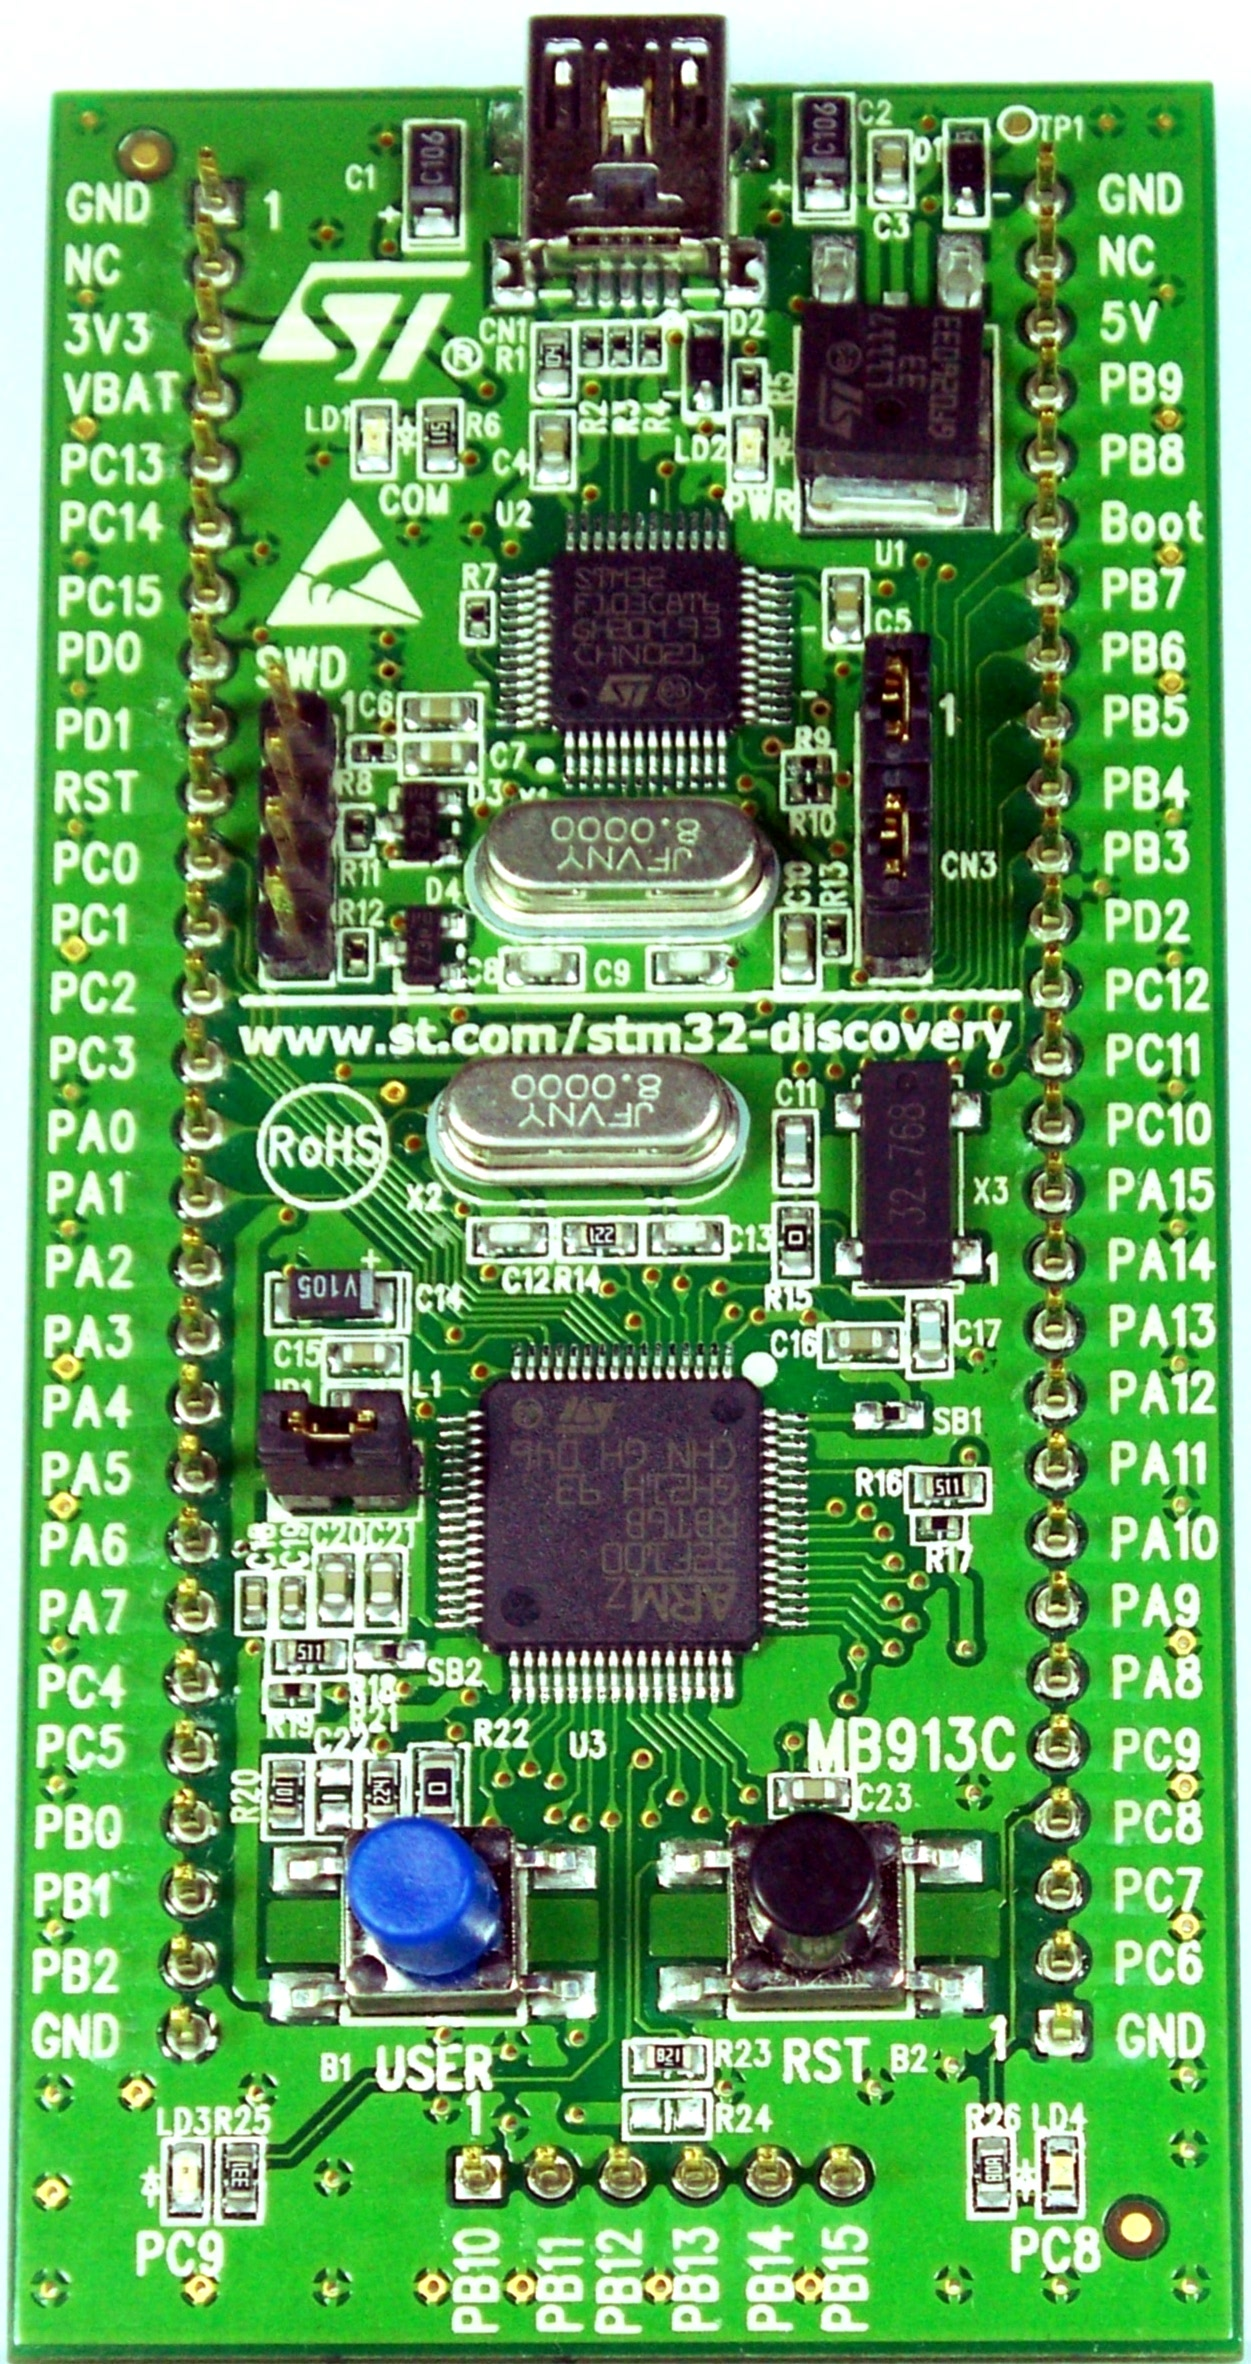
\includegraphics[width=.25\textwidth]{images/stm32_discovery_board.jpg}
\caption{Vývojová doska STM32 vl Discovery}
\label{obr2}
\end{center}
\end{minipage}
\end{center}
\end{figure}

Doska Discovery kit obsahuje len minimum periférií. K dispozícií su dve LED a dve tlačítka (užívateľské a reset). Dobrá vlastnosť je vyvedené programovacie rozhranie na dip lištu. To umožňuje použiť túto dosku na programovanie externe osadených mikrokontrolérov. Veľkou nevýhodou je neprítomnosť UART/USB rozhrania, ktoré by zjednodušilo ladenie. Práve za tým účelom bola navrhnutá testovacia doska. Je vybavená väčšími možnosťami pripojenia periférií. Jedna dutinková lišta je vybavená UART rozhraním aj napájaním. Na toto rozhranie je možné priamo zasunúť prevodník USB/UART s FT232 \cite{usb_uart}. Je potrebné dodržať 3.3V napäťové úrovne. Testovacia doska ďalej obsahuje sadu tlačidiel a LED diód. K dispozícií je aj konektor pre SD kartu. Pre jedoduché ovládanie malých motorov, je na doske prítomný aj mostík, umožňujúci budiť dva motory. Vďaka použitiu low drop stabilizátora je dosku možné napájať aj z jediného li-pol článku. Využitie jeho kapacity však zďaleka nebude najlepšie.

\begin{figure}[ht]
\begin{center}
\begin{minipage}{1.1\linewidth}
\begin{center}
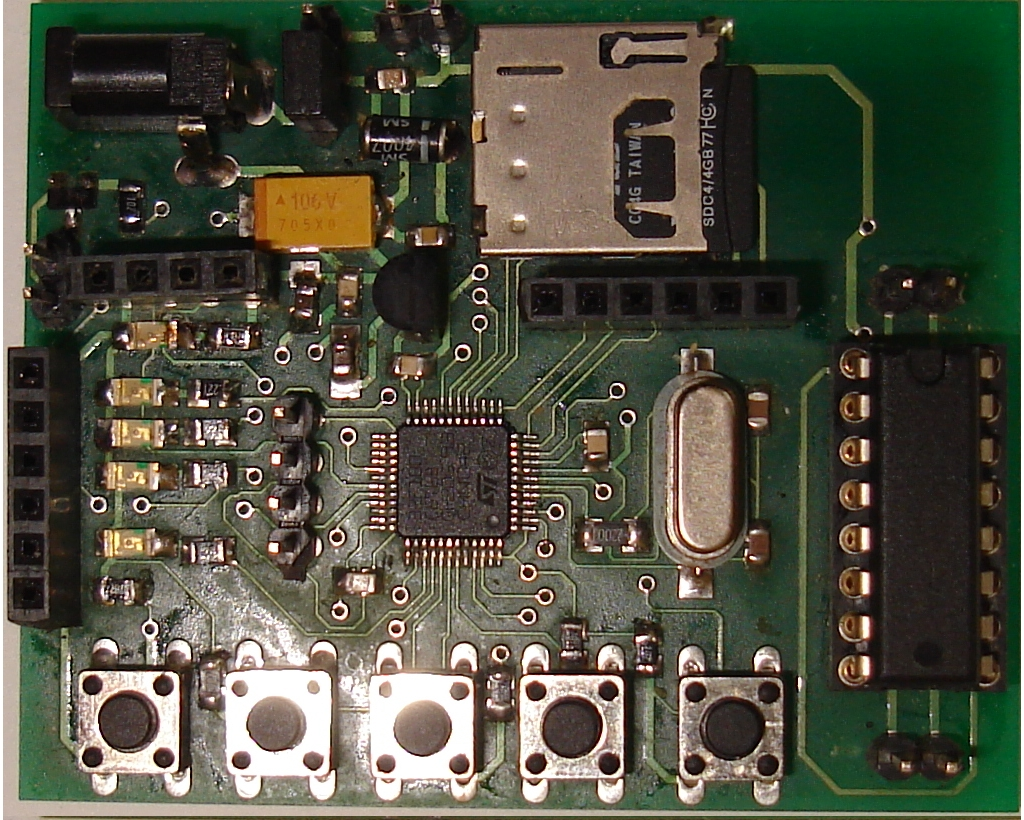
\includegraphics[width=.35\textwidth]{images/test_board.jpg}
\caption{Testovacia doska}
\label{obr2}
\end{center}
\end{minipage}
\end{center}
\end{figure}

\subsection {Stellaris Launchpad}

Pre testovanie funkcionality systému aj na jadre Cortex M4, bola zvolená vývojová doska Stellaris Launchpad firmy Texas Instruments \cite{stellaris_kit}.

\begin{figure}[ht]
\begin{center}
\begin{minipage}{1.1\linewidth}
\begin{center}
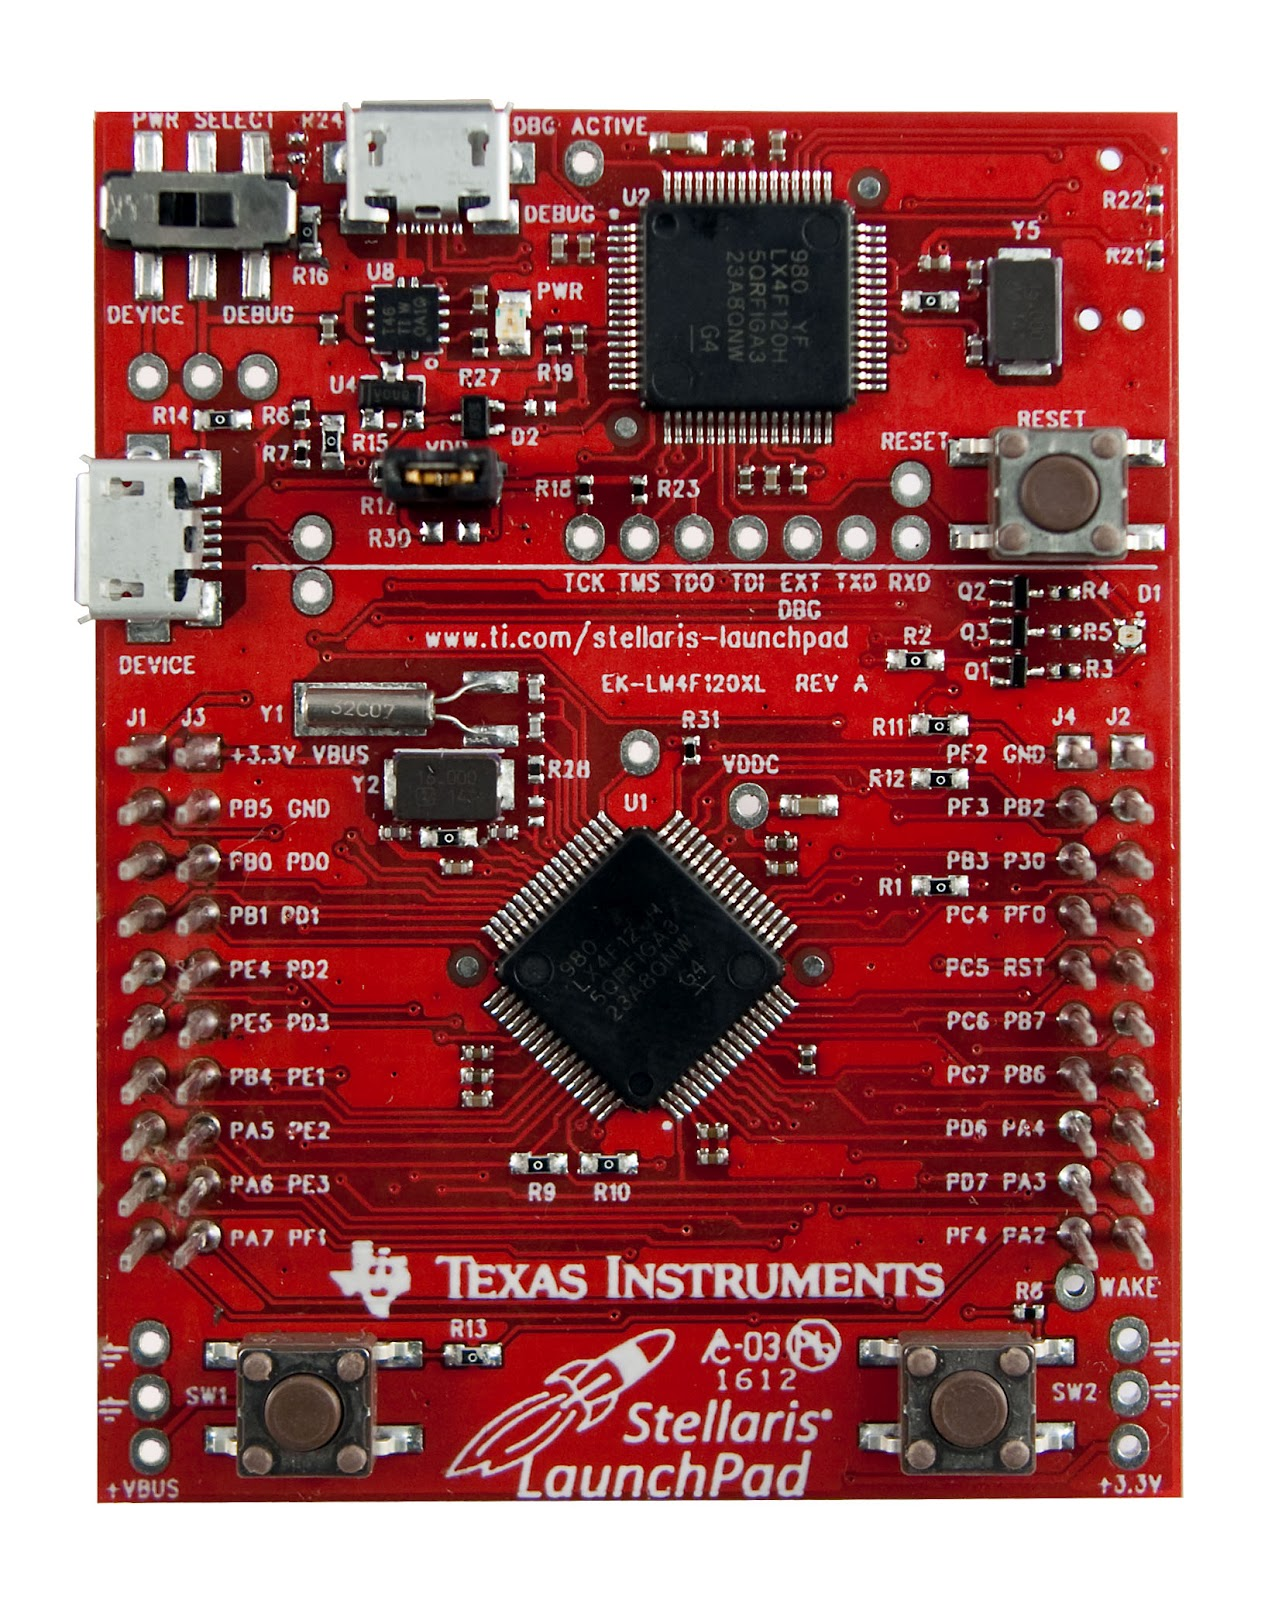
\includegraphics[width=.35\textwidth]{images/launchpad_lm4f120.jpg}
\caption{Vývojová doska Stellaris Launchpad}
\label{obr2}
\end{center}
\end{minipage}
\end{center}
\end{figure}

Doska je vybavená troma tlačidlami. Zaujímavosťou je prítomnosť RGB led diódy. Po pripojení do počítača, sa vytvorí nový sériový port, najčastejšie ako /dev/ttyACM0. Tento fakt veľmi zjednodušuje ladenie aplikácie.

\section {Testovanie jadra}

Na korektné otestovanie jadra je v adresári \textbf{usr/threads} program, ktorý vytvára a ničí vlákna. Tento proces prebieha v cykle a umožňuje tak určit, či sa vlákno správne vytvorí aj ukončí. Dôležitým parametrom je aj čas prepnutia kontextu, z ktorého možno odvodiť záťaž mikroprocesora jadrom systému. Za týmto účelom bol vytvorený dvojvláknový program. Jedno vlákno neustále zapína led. Druhé tú istú led neustále vypína. V obsluhe prerušenia od časovača sa ihneď po uložení kontextu zapne druhá led a tesne pred obnovou kontextu sa led vypne. Pripojením dvojkanálového osciloskopu na dve led, je možné určiť potrebné časy.

\begin{figure}[ht]
\begin{center}
\begin{minipage}{1.1\linewidth}
\begin{center}
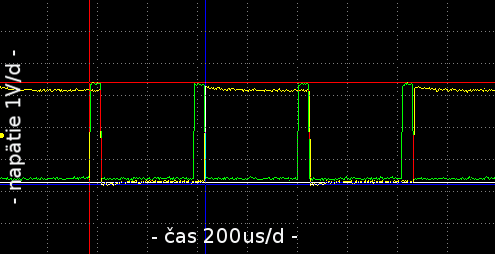
\includegraphics[width=.7\textwidth]{images/cm3_context_switch_02_.png}
\caption{Priebehy napätí pri meraní doby prepnutia kontextu jadra Cortex M3}
\label{obr2}
\end{center}
\end{minipage}
\end{center}
\end{figure}

Frekvencia prepínania kontextu bola zámerne zvýšená na 2kHz, aby sa záznam vošiel na obrazovku. Doba prepnutia kontextu je doba zeleného priebehu. Nameraný čas je 46us pri frekvencií jadra 24MHz. To je približne 1100 inštrukcií (orientačný údaj). 

Pre jadro Cortex M4, taktované na 80MHz bol čas prepnutia kontextu 12us. Pomer rýchosti jadier je 3.33, rovnako ako pomery časov prepnutí kontextu. Merania teda zodpovedajú teoretickému predpokladu - na prepnutie kontextu totiž nie sú využité žiadne špeciálne inštrukcie typické pre jadro Cortex M4.

\begin{figure}[ht]
\begin{center}
\begin{minipage}{1.1\linewidth}
\begin{center}
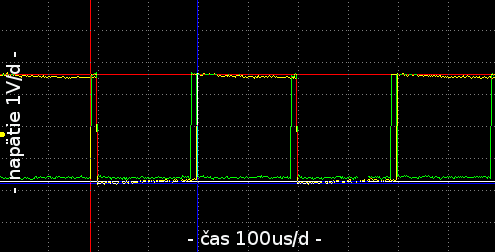
\includegraphics[width=.7\textwidth]{images/cm4_context_switch_02_.png}
\caption{Priebehy napätí pri meraní doby prepnutia kontextu jadra Cortex M4}
\label{obr2}
\end{center}
\end{minipage}
\end{center}
\end{figure}

Treba poznamenať, že vzhľadom na neustále zlepšovanie programu systému, sú súčasné hodnoty už lepšie. Došlo k vyňatiu jedného cyklu, čím sa výrazne znížil potrebný počet inštrukcií a zvýšila efektivita využitia procesora.

\newpage
\section {Testovanie zámkov}

Pre korektné testovanie vstupu a výstupu z kritických sekcií, slúži program \textbf{usr/lock}. Vytvoria sa tri vlákna a každé píše do terminálu svoj text. Funkcia eprint prebieha atomicky. Jednotlivé riadky by teda mali byť zobrazené korektne. V prípade vyhodenia knižnice lock.c, bude text riadkov rozhádzaný a prepletený s inými vláknami. Funguje to vďaka tomu, že UART jednotka je vybavená vyrovnávacou pamäťou a preto znesie náhly nápor dát. Situáciu dobre vystihuje nasledujúci obrázok z terminálového výstupu systému.


\begin{figure}[ht]
\phantom.\hfill
%
\begin{minipage}{0.45\linewidth}
\begin{center}
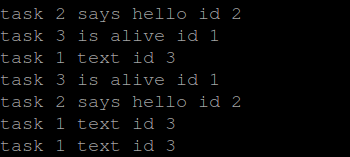
\includegraphics[width=0.9\textwidth]{images/atomic_.png}
\caption{S využitím mutexu}
\label{obrL1}
\end{center}
\end{minipage}
%
\hfill 
%
\begin{minipage}{0.45\linewidth}
\begin{center}
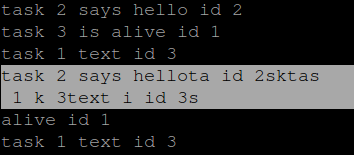
\includegraphics[width=0.9\textwidth]{images/no_atomic_.png}
\caption{Neošetrené použitie}
\label{obrP1}
\end{center}
\end{minipage}
%
\hfill\phantom.
\end{figure}


\section {Testovanie správ}

Systém správ bol testovaný na aplikácií klient-server. Dve vlákna neustále posielajú svoju požiadavku serveru. Požiadavkou bola inkrementácia položky msg.data. Každý klient začal s inou počiatočnou hodnotou. Jeden na 0, druhý na 1. Očakávaný výstup v termináli je potom, že jedon vlákno vypisuje párne a druhé nepárne čísla. Uvedený program je v adresári \textbf{usr/messages}. Pre otestovanie možnosti posielať komplexnejšie dáta, je určená aplikácia cli, v adresári \textbf{usr/cli}. Aplikácia ukazuje prácu so súborovým systémom. Ovládač súborového systému je prítomný ako samostatné vlákno, čakajúce na správu - požiadavka na výpis adresára alebo čítanie súboru. Samotný prenos správy je riešený pomocou pretypovania ukazovateľa a využitia synchrónneho poslania požiadavky serveru.
\newpage
\begin{figure}[ht]
\begin{center}
\begin{minipage}{1.1\linewidth}
\begin{center}
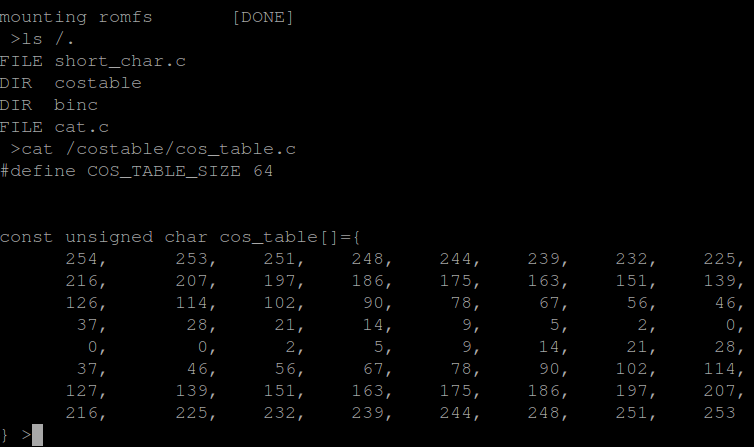
\includegraphics[width=.7\textwidth]{images/romfs_.png}
\caption{Výpis obsahu súboru costable.c}
\label{obr2}
\end{center}
\end{minipage}
\end{center}
\end{figure}

Na obrázku je znázornené použitie súborového systému. Príkazy sú podobné ako v systéme Linux. Treba poznamenať, že primárnym cieľom nebolo vytvorenie komfortného príkazového riadka. Toto rozhranie je implementované najmä za účelmi kvalitného testovania. Ponúkaná funkčnosť je preto veľmi strohá. Implementovať vlastné užívateľské rozhranie však nepredstavuje závažný problém.


 % testovanie OS
\chapter{Aplikačné použitie operačného systému}

Táto kapitola popisuje použitie operačného systému koncovým užívateľom (programátorom) vlastnej aplikácie. Snahou je umožniť komfortný, rýchlejší a modulárny vývoj aplikácie. Celý proces je demonštrovaný na sade jednoduchých príkladov, ktoré ukážu vlastnosti operačného systému. Najmä pre menej skúseného užívateľa môže byť kompilácia systému zo zdrojových kódov prekážkou, preto kapitola začína časťou popisujúcou samotnú kompiláciu a nastavenie arm gcc kompilátora.

\section{Kompilácia arm-gcc}

Celý systém je vyvýjaný s použitím balíka \textbf{arm-gcc} v prostredí GNU Linux, ktorý predstavuje sadu nástrojov pre tvorbu binárnych súborov, bežiacich na architektúre arm. Balík je možné stiahnúť, napr. z git repozitárov \cite{arm_summom_git}. Po rozbalení arhívu stačí spustiť skript : 
{\small
\begin{verbatim}
./summon-arm-toolchain
\end{verbatim}
}


Následne sa spustí kompilácia niekoľkých častí gcc kompilátora. Ďalšie potrebné súbory sa stiahnú automaticky. Po ukončení kompilácie sa vytvorí v domovskom adresári adresár sat, ktorý obsahuje pripravený kompilátor pre ARM jadro.
 
Pre uloženie binárneho súboru do flash pamäte mikrokontroléra, je potrebné stiahnúť \textbf{stlink} \cite{stlink} a \textbf{lm4flash} \cite{lm4_flash}. Stlink spolupracuje s vývojovou doskou STM Discovery Kit a umožňuje programovať mikrokontroléry z radu STM32. Program lm4flash poskytuje rozhranie s doskou TI Stellaris Launchpad a umožňuje programovať mikrokontroléry LM4F120 a príbuzné. Pre kompiláciu oboch stačí spustiť make all a prebehne kompilácia nástrojov. Kvôli urýchleniu práce, je vhodné urobiť jednoduché skripty pre ukladanie do flash pamäte :

{\small
\begin{verbatim}
sudo ~/bin/stlink/flash/st-flash write main.bin 0x8000000
\end{verbatim}
}

{\small
\begin{verbatim}
sudo ~/bin/lm4tools/lm4flash/lm4flash main.bin
\end{verbatim}
}

Všetky použité skripty predpokladajú, že sú uložené v adresári bin, ktorý je umiestnený v domovskom adresári :
{\small
\begin{verbatim}
 $(HOME)/bin
\end{verbatim}
}

Do tohto adresára je vhodné umiestniť aj kompilátor a premenovať ho na arm-none-eabi. Na komfortný vývoj sa pre mikrokontroléry Stellaris odporúča použitie knižnice Stellaris Ware. Po bezplatnej registrácií, je možné ju stiahnúť na tejto adrese \cite{stellaris_ware}.


\section{Štruktúra adresárov operačného systému}

Systém je organizovaný do niekoľkých adresárov. Pomenovanie je prevzaté z prostredia Linux a majú aj podobný význam. Adresárová štruktúra systému je nasledujúca :

\begin{figure}[ht]


\dirtree{%
.1 /.
.2 \textcolor{cyan}{bin}.
.2 \textcolor{red}{common}.
.3 \textcolor{black}{stellaris}.
.3 \textcolor{black}{stm32}.
.3 \textcolor{black}{stmdiscovery}.
.2 \textcolor{red}{kernel}.
.2 \textcolor{blue}{lib}.
.2 \textcolor{red}{startup}.
.2 \textcolor{green}{usr}.
.3 cli.
.3 discovery\_kit\_demo.
.3 hello\_world.
.3 locks.
.3 messages.
.3 threads.
}

\end{figure}

Pre sprístupnenie systému čo najširšiemu počtu záujemcov sú zdrojové kódy k dispozícií na servery SourceForge. Odkaz pre stiahnutie zdrojových súborov je tu \cite{suzuha_source}.

\subsection{Koreňový adresár}




Obsahuje samotné makefiles pre kompiláciu systému. Podľa voľby architektúry sa vyberie jeden z dvoch dostupných :
{\small
\begin{verbatim}
make -f stm32_make -B
\end{verbatim}
}

{\small
\begin{verbatim}
make -f lm4f_make -B
\end{verbatim}
}

Ak sú správne nastavené cesty ku kompilátoru a knižniciam prebehne kompletné skompilovanie celého systému. Parameter -f uvádza názov makefile, nakoľko sú použité neštandartné názvy. Parameter -B informuje program make, že má vykonať kompletnú kompiláciu bez ohľadu na to, či sú objektové binárne súbory už aktuálne.
Cesty ku knižniciam a kompilátoru sú uvedené v prvých riadkoch makefile, aby bolo možné jednoducho meniť umiestnenie kompilačných nástrojov na disku :

{\small
\begin{verbatim}
STELLARIS_WARE_PATH = $(HOME)/bin/stellarisware
COMPILER_PATH = $(HOME)/bin/arm-none-eabi/bin
\end{verbatim}
}

V koreňovom adresári sa ďalej nachádza konfiguračný súbor systému : \textbf{configure.h}. V ňom prebieha základná konfigurácia systému. Najdôležitejšia je voľba architektúry mikrokontroléra. Slúžia k tomu nasledujúce dva riadky. Len jeden z nich môže byť nezakomentovaný. Podľa tejto voľby sa vyberajú príslušné knižnice a moduly systému.

{\small
\begin{verbatim}
#define CPU_LM4F		1	/*choose cpu LM4F*/
#define CPU_STM32		1	/*choose cpu STM2*/
\end{verbatim}
}

Ďalší parameter špecifikuje frekvenciu systémového časovača : 
\begin{verbatim}SYS_TICK_PERIOD\end{verbatim} 
je závislý od taktovacej frekvecie a ovplyvňuje periódu spúšťania časovača systick - perióda volania prepínania úloh.

Maximálny počet definovaných úloh v systéme je možné špecifikovať nasledujúcim parametrom.
\begin{verbatim}TASK_MAX_COUNT N\end{verbatim}

Pre režim zníženej spotreby je možné povoliť parameter : 
\begin{verbatim}LOW_POWER_MODE\end{verbatim}
Samotná funkcia režimu zníženej spotreby je však hardvérovo aj aplikačne závislá, jej implementácia zostáva preto na užívateľovi. V systéme je definovná volaním inštrukcie "wfe" (viac súbor kernel/kernel.c).

Experimentovať je možné voľbou rôznych plánovacích algoritmov. Súčasná verzia má dva, pričom testovanie sa najviac zameriava na prioritný plánovač a round robin algoritmus je uvažovaný len ako núdzové riešenie. V systéme sa preto odporúča nechať prioritný plánovač.
{\small
\begin{verbatim}
#define SCHED_PRIORITY		1
\end{verbatim}
}


Súbor \textbf{common.h} obsahuje odkazy na všetky potrebné hlavičkové súbory. Zjednodušuje tak vývoj aplikácie, v ktorej potom stačí vložiť len tento jeden súbor, ktorý vyrieši všetky systémové závislosti.

Súbor \textbf{main.c} obsahuje vstupný bod do programu. Je možné v ňom definovať dodatočnú inicializáciu, pokiaľ systém ešte nebeží. Prebieha v ňom inicializácia vytvorenia hlavného systémového vlákna : 
{\small
\begin{verbatim}
main_thread
\end{verbatim}
}

Ak sa to nepodarí, končí systém zastavením a vypísaním chybového hlásenia - nula vláknový systém nemá zmysel spúšťať. Ak sa to podarí, systém začne vykonávať program hlavného vlákna. Na toto vlákno je kladená jediná odlišná požiadavka : nesmie byť ukončené. Po jeho ukončení (a/alebo ukončení všetkyçh ostatných vlákien - záleží od plánovača), nie je správanie sa sytému definované.

V hlavnom adresári sa ďalej nachádza súbor s licenciou a súbor TODO, ktorý obsahuje body, ktoré častí systému je vhodné upraviť, prípadne odstrániť chyby.

\subsection{Adresár bin}

Tento adresár obsahuje výsledný binárny súbor, pripravený na nahratie do mikrokontroléra. Tento súbor je z dôvodu automatizácie skriptom pomenovaný \textbf{main.bin}. Na nahratie slúžia skripty :
{\small
\begin{verbatim}
write_lm4
write_stm32
\end{verbatim}
}

Treba poznamenať, že skripty nevedia rozlíšiť správnosť súboru \textbf{main.bin}, najmä to, pre ktorú architektúru bol kompilovaný. Je na užívateľovi aby spustil správny skript, pre konkrétny mikrokontrolér. Väčšinou to npredstavuje problém a program jednoducho napôjde. Závažnejšia situácia nastane, ak pre chybnú interpretáciu programu dôjde k cyklickému prepisovaniu flash pamäte (čo môže viesť k jej zničeniu).

Pre účely ladenia je v tomto adresári obsiahnutý súbor \textbf{\textbf{assembler.lss}}. Obsahuje extrahovaný strojový kód preložený do jazyka symbolických adries, doplnený komentármi zo zdrojových súborov. Umožňuje tak vidieť výsledok prekladu a v prípade závažného problému pomôcť pri odlaďovaní.

Linker potrebuje pre správne prepočítanie adries, tzv. linkovací skript. Je závislý najmä od veĺkosti a usporiadania pamäte kontrétneho mikokontroléra. Skript obsahuje informácie o veľkostiach pamäte a kde pamäť začína. Ďalej sa v ňom nachádzajú informácie o poziícií a vlastnosti pamäte - flash je len na čítanie a ram má atribút pre čítanie aj zápis.
Tieto skripty sú v nasledujúcich dvoch súboroch :
{\small
\begin{verbatim}
lm4f.ld
stm32.ld
\end{verbatim}
}

Celý program je rozdelený z pohĺadu linkera na tzv. sekcie. Vykonateľný program a konštantné premenné sú uložené v sekcií text. V skripte jej začiatok a koniec označujú symbolické názvy :
{\small
\begin{verbatim}
_text
_etext
\end{verbatim}
}
Túto skutočnosť je možné využiť, napr. pri tvorbe bootloadera.

Oblasť data zahŕňa všekty inicializované premenné.
Pre systémového programátora je najdôležitejšia sekcia bss. Symbolické názvy
{\small
\begin{verbatim}
_bss
_ebss
\end{verbatim}
}
Je možné použiť na alokáciu vlastnej pozície zásobníka. Prípadne pre vytvorenie vlastnej funkcie malloc.

\subsection{Adresár startup}

V tomto adresári sú obsiahnuté štartovacie sekvencie mikrokontroléra. Je to hardvérovo závislá časť, preto sa nachádzajú v oddelených súboroch.
{\small
\begin{verbatim}
startup_lm4f.c
startup_stm32.c
\end{verbatim}
}

Z pohľadu užívateľa je zaujímavá najmä definícia obslúh prerušení. Súbor obsahuje pole konštánt, predstavujúce adresy funkcií obslúh prerušení. Všetky prerušenia po SysTick vrátane, sú spoločné pre jadrá Cortex. Oatatné prerušenia sú závislé na voľbe výrobcu a akými perifériami je mikrokontrolér vybavený. Väčšina prerušení je definovaná ako IntDefaultHandler, čo pri nesprávne vyvolanom prerušení (programátorska chyba, nedefinovaný skok ...), spôsobí zastavenie v nekonečnej slučke.

Po resete mikokontroléra, sa začne vykonávať program od funkcie ResetISR. Tá predstavuje vstupný bod do celého programu. Obvykle v nej prebieha inicializácia premenných : skopírovanie nenulových hodnôt do ram a nulovanie sekcie bss. Ďalej sa môže vykonať inicializácia koprocesora, prípadne inej, kritickej periférie.

Po ukončení inicializácie sa volá funkcia \textbf{int main()} a riadenie je ponechané aplikácií.

\subsection{Adresár common}

Pre zabezpečenie jednoduchej prenositeľnosti, je k dispozícií tento adresár. Obsahuje hardvérovo závislé knižnice - najmä definície registrov. Umožňuje definovať hardvér vývojovej dosky (pomocou súboru common.c) a vytvoriť tak najnižšiu formu abstrakcie. Kvôli nejednoznačnej definícií typu int sa tu nachádzajú súbory, ktoré definujú typy, ako u32 alebo i32 a odstraňujú závislosť na kompilátore. Tieto typu sú používané v celom systéme.

Súbor \textbf{common.h} vkladá súbor podľa použitej dosky a preriférií :
{\small
\begin{verbatim}
stm32.h
stellaris_aunchpad.h
\end{verbatim}
}

Oba obsahujú odkazy na knižnice a ovládanie periérií (led a tlačítka).
Funkcie najnižšej úrovne sú :
{\small
\begin{verbatim}
void common_init();
void delay_loops(u32 loops);
void led_on(u32 led);
void led_off(u32 led);
u32 get_key();
\end{verbatim}
}

\subsection{Adresár kernel}

V tomto adresári sa nachádza samotné jadro operačného systému. Súbor \textbf{kernel.h} obsahuje definície systémových konštánt a najdôležitejších sytémových funkcií. Tie sú nevyhnutné najmä pre tvorbu vlastnej knižnice. Z funkcií, ktoré priamo ovplyvňujú systém, sú to :
{\small
\begin{verbatim}
void sched_off();	/*zakázanie prerušení*/
void sched_on();	/*povolenie prerušení*/
void sched_next();	/*okamžité prepnutie na ďalšiu úlohu*/
void low_power_mode();	/*vstúpenie do režimu spánku*/
void set_wait_state();  /*uspí aktuálne vlákno*/
void wake_up_threads(); /*zobudí všetky vlákna*/
\end{verbatim}
}

Použitie funkcií, zakazujúce a povoľujúce prerušenie, je treba dôkladne zvážiť a používať len v nevyhnutných prípadoch. Funkcia pre okamžité prepnutie umožňuje urýchliť reakciu systému a nezaťažovať jadro zbytočným čakaním. Vo funkcii pre vstup do režimu zníženej spotreby, je možné definovať aplikačne závislý režim šetrenia energie.

Najdôležitejšia funkcia jadra je :
{\small
\begin{verbatim}
u32 create_task(void *task_ptr, u32 *s_ptr, u32 stack_size, u16 priority);
\end{verbatim}
}

Umožňujúca vytvorenie nového vlákna.

\subsection{Adresár lib}

Všetky zdieľané knižnice je vhodné uložiť do tohto adresára. Väčšina knižníc je na sebe nezávislá. Prioritné postavenie má knižnica lib.c, ktorá vykonáva inicializáciu všetkých ostatných knižníc (ak ju treba) volaním \textbf{kniznica\_init()}. 

\begin{itemize}
	\item lock.h : knižnica zabezpečuje vstup do kritických sekcií pomocou zámkov (mutex).
	\item mesages.h : systém predávania správ medzi vláknami (bez fronty).
	\item messages\_f.h : systém predávania správ (s frontou správ).
	\item sw\_timer.h : knižnica softvérových časovačov.
	\item uart.h : nízkoúroňové riadenie uart jednoty (prečítanie/poslanie znaku).
	\item std\_io.h : knižnica štandartného vstupu/výstupu.
\end{itemize}

\subsection{Adresár usr}

Do tohto adresára sa umiesťuje samotná implementácia aplikácie. V súbore usr.h je definované pole pre zásobník hlavnej úlohy a referencia na ňu. Veľkosť zásobníka je možné podľa potreby pozmeniť. V súbore \textbf{usr.c} je vložený odkaz na hlavný program aplikácie (napr. hello\_world/threads.c). V samotnom súbore threads je potom definícia funkcie \textbf{main\_thread()}. 
Obsah adresára usr je možné modifikovať podľa potreby aplikácie. Podmienkou je len prítomnosť hlavného vlákna a definícia jeho zásobníka. Pre väčšie projekty je vhodné vytvoriť samostatný makefile pre aplikačnú casť.

\section{Tvorba aplikácie}

\subsection{Blikanie led}
Ukážková aplikácia vytvorí dve vlákna. Každé vlákno ovláda svoju led. Periodicky ju zapína a vypína. Vďaka rôznym čakacím intervalom pôsobi blikanie dvoch led zdanlivo chaoticky. Tento program nevyžaduje žiadne knižnice systému, využíva sa len obsah z \textbf{common/common.h}. Vo funkcii \textbf{int main()} je možné zakomentovať výpisy do terminálu a vyhnúť sa tak použitiu \textbf{std\_io.h} aj \textbf{uart.h} knižníc.
{\small
\begin{verbatim}
void task2()
u32 task2_stack[32];

void main_thread() {
 create_task(task2, task2_stack, sizeof(task2_stack), PRIORITY_MAX);

 while (1) {
   led_on(1);	/*zapne led 1*/
   delay_loops(1000000);
   led_off(1);	/*vypne led 1*/
   delay_loops(10000000);
 }
}

void task2() {
 while (1) {
   led_on(2);	/*zapne led 2 */
   delay_loops(6000000);
   led_off(2);	/*vypne led 2*/
   delay_loops(10000000);
  }
}
\end{verbatim}
}

Hlavné vlákno \textbf{main\_thread}vytvorí druhé vlákno volaním funkcie jadra \textbf{create\_task}. Parametrami je ukazovateľ na hlavnú funkciu vlákna, ukazovateľ na zásobník vlákna, veľkosť zásobníka a priorita procesu. Dôležitým faktom je nutnosť použiť na zásobník pole ako globálnu premennú - kompilátor ma inak snahu realizovať pole lokálne a relatívne adresované. To sposobí nefunkčnosť systému.


\subsection{Časovače a eprintf}
S malou úpravou a vložením knižníc je možné využiť programový časovač \textbf{sw\_timer.h}. Časovač sa inicializuje na 250ms a spustí sa odpočet. Po dosiahnutí nuly, funkcia \textbf{wait\_for\_timer()} skončí. Vlákno zároveň pomocou funkcie eprintf vypisuje na terminál správu o svojej existencií. Knižnica eprintf využíva možnosti mutexov a uart, treba preto použiť aj knižnicu \textbf{lock.h} a \textbf{uart.h}. Treba poznamenať, že časovač má maximálny časový interval daný 32 bitovou hodnotou. Pri volaní 1000-krát za sekundu je maximálna doba čakania 49.7 dňa.

{\small
\begin{verbatim}
 while (1) {
   eprintf("thread 01\n");

   led_on(1);	/*zapne led 1*/
   timer_start(250, SW_TIMER1);	/*nastavenie časovača*/
   wait_for_timer(SW_TIMER1);   /*čakanie na časovač*/

   led_off(1);	/*vypne led 1*/
   timer_start(250, SW_TIMER1);	/*nastavenie časovača*/
   wait_for_timer(SW_TIMER1);  /*čakanie na časovač*/
 }
\end{verbatim}
}

Knižnica \textbf{sw\_timer.h} poskytuje osem softvérových časovačov. K presnému časovaniu používa jeden hardvérový časovač, nastavený na periodické vyvolávanie prerušenia - 1ms. Preto funkcia  wait\_for\_timer nebude nikdy presnejšia ako 1ms a pre malé časové intervaly môźe byť chyba neúnosná. Knižnica je preto vhodná najmä na dlhšie časové intervaly, ktoré nie sú kritické na presnosť.

Funkcia eprintf poskytuje možnosti formátovaného výstupu na terminál. Z dôvodu šetrenia zdrojov mikrokontroléra, v nej nie je implementovaná možnosť výpisu čísel v pohyblivej rádovej čiarke. Podporované formáty sú \%i \%u \%x \%c \%s.


\subsection{Zámky}

V prípade viacvláknovej aplikácie sa často vyskytuje situácia riešenia vyhradeného prístupu k určitej periférií, prípadne časti programu. Je kladená požiadavka, aby druhé vlákno do tejto kritickej sekcie nemohlo vstúpiť, kým druhé vlákno sekciu neopustí. Pre veľmi jednoduché prípady je možné použiť zakázanie a povolenie prerušenia :
{\small
\begin{verbatim}
void sched_off();	/*zakázanie prerušenia*/
void sched_on();	/*povolenie prerušenia*/
\end{verbatim}
}
Toto riešenie je však veľmi nebezpečné a ťažkopádne : pokým sú zakázané prerušenia je systém zastavený, vlákna nie sú prepínané a môže dôjsť k narušeniu splnenia podmienok reálneho času. Je preto vhodné len na veľmi rýchle sekcie programu. Príkladom sú napr. prístupy ku globálnym premmenným.

Všetky ostné prípady je potrebné riešiť knižnicou \textbf{lock.h}. Použité pojmy lock sú bližšie skutočnej úlohe, ako často uvádzané pojmy mutex alebo semafór. Knižnica používa dve funkcie, pre zamykanie a odomykanie prístupu k zariadeniu :
{\small
\begin{verbatim}
void lock_dev(u32 dev_flags);		/*vstup do kritickej sekcie/
void ulock_dev(u32 dev_flags);		/*odchod z kritickej sekcie*/
\end{verbatim}
}
Premenná \textbf{dev\_flags} obsahuje bitovú masku pre zamykanú perifériu/časť programu. Je možné použiť 32 rôznych sekcií, vrátane ich kombinácií - naraz je možné zamknúť viac zdrojov. Situáciu je dobré ilustrovať na príklade :
{\small
\begin{verbatim}
lock_dev(LOCK_UART_TX); /*LOCK_UART_TX == (1<<0)*/
send_uart(c);		/*pošle byte*/
ulock_dev(LOCK_UART_TX);/*uvoľnenie kritickej sekcie*/
\end{verbatim}
}
V tomto prípade sa zamyká len 1 bit, pre zariadenie vysielača sériovej linky. Niekedy je vŠak vhodné uzamknúť viac zariadení naraz, umožní to vyhnúť sa deadlocku spôsobeného nesprávnym volaním zámkov. Zamknutie prístupu k viacerým zariadeniam naraz vyzerá nasledovne :
{\small
\begin{verbatim}
lock_dev(LOCK_UART_TX|LOCK_UART_RX); /*uzamknutie prístupu*/
c = get_uart();			     /*prečítanie znaku z uart*/
send_uart(c);			     /*poslanie znaku späť*/
ulock_dev(LOCK_UART_TX|LOCK_UART_RX);/*odomknutie prístupu*/
\end{verbatim}
}




\subsection{Systém správ}

Architektúra klient-server, poskytuje robustné modulárne riešenie. Pre správnu funkciu vyžaduje použitie systému správ, poskytujúci primeranú mieru abstrakcie komunikácie medzi vláknami. Túto možnosť ponúka knižnica \textbf{messages.h}m, prípadne novšia verzia s frontou \textbf{messages\_f.h}. Pre bezpečné funkcie systému sa odporúča používať systém správ s frontou. 

Najprv sa vlákno registruje na prácu so správami, pod symbolickým menom MSG\_SERVER. Toto meno musí byť známe aj všetkým klientom. Následne sa vytvorí druhé vlákno - predstavujúce napr. klienta.

{\small
\begin{verbatim}
 msg_register(MSG_SERVER);
 create_task((void*)task2, task2_stack, sizeof(task2_stack),PRIORITY_MAX);
\end{verbatim}
}

Server v hlavnej slučka čaká na správu :
{\small
\begin{verbatim}
 while (1) {
  msg_get(&msg);		/*čakanie na správu*/
  msg.data+= 2;		       /*zmena dát*/
  msg.destination= msg.source; /*príprava na odpoveď*/
  msg.source = MSG_SERVER;     /*označenie odosielateľa*/
  /* msg.size = msg.size;	veľkosť bez zmeny*/
  msg_raise_async(&msg);       /*poslanie odpovede*/
 }
\end{verbatim}
}

Funkcia \textbf{msg\_get()} čaká na príjem správy. Po príjme správy, sa naplní štruktúra správy. Server ju teraz môže ľubovoľne vyhodnotiť. V ukážkovom príklade sa hodnota data zväčší o dva. Meno príjemcu sa naplní menom odosielateľa. Meno odosielateľa sa aktualizuje na meno servera. Veľkosť správy sa necháva bez zmeny. Následne sa volaním funkcie \textbf{msg\_raise(\&msg)} odošle odpoveď klientovi.
Dôležitým faktom je, že funkcia \textbf{msg\_raise()} čaká, pokiaľ klientské vlákno správu neprevezme. Naproti tomu, funkcia \textbf{msg\_raise\_async()} správu vloží do fronty a ihneď končí. Jej použitie je preto vhodné pre serverovú časť - predpokladá sa nespoľahlivosť klienta, ktorý z rôznych príčin nemusí prevziať správu. Naopak, synchrónne volanie msg\_raise je vhodné pre klienta, kde sa predpokladá plne funkčný server a záruka prijatia správy.

Vlákno klienta je realizované veľmi podobne ako server :
{\small
\begin{verbatim}
 struct sMsg msg;
 msg_register(MSG_CLIENT_A);  /*registrácia na prácu so správami*/
 msg.data=0;		      /*inicializácia dát*/	
 while (1) {
  msg.size=4;		     /*veľkosť správy 4byty*/
  msg.source=MSG_CLIENT_A;   /*vyplnenie zdroja*/
  msg.destination=MSG_SERVER;/*cieľ správy - server*/

			     /*výpis stavu správy*/
  eprintf("client id %u  server id %u | data : %u\n", 
	   msg.source, msg.destination, msg.data);
  delay_loops(1000000);
	 
  msg_raise(&msg); 	    /*poslanie požiadavky na server*/
  msg_get(&msg); 	    /*čakanie na odpoveď*/
 }
 }
\end{verbatim}
}

Opäť je použitá registrácia pod symbolickým menom, v tomto prípade stačí, aby bolo odlišné od mena servera. Pre väčší počet klientov sa však vyžaduje, aby meno bolo v systéme jedinečné. Klientské vlákno pošle správu serveru. Ten inkrementuje hodnotu msg.data o dva a pošle späť. Klient vypíše na terminál stav správy : odosielateľ, príjemca a obsah položky data.

Dôležitým faktom, je možnosť položku data pretypovať na ľubovoľný iný dátový typ. Podľa jeho veľkosti treba upraviť položku size. Systémom správ je tak možné pomocou ukazovateľov prenášať ľuboboľné dátové typy. Mimoriadnu pozornosť je potrebné venovať atomicite operácií : odosielaná dátová štruktúra nesmie byť menená, pokým nepríde odpoveď od servera.


\section{Ďalšie príklady aplikácie}

V adresári usr sa nachádzajú rôzne testovacie príklady pre použitie operačného systému.

\subsection{Hello\_world}
Ukážka jednoduchého trojvláknového programu. Aplikácia postupne bliká troma led, každá led je riadená svojím vláknom. Nevyžaduje sa žiadna knižnca zo sekcie lib.

\subsection{Timers}
Podobne ako v predošlom prípade, na riedenie časových intervalov je však použitá knižnica \textbf{sw\_timer.h}. Frekvenciu blikania je teda možné nastaviť s milisekundovým rozlíšením.

\subsection{Locks}
Vlákna vypisujú správy do terminálu s použitím funkcie eprintf (knižnica std\_io.h). Funkcia eprintf prebehne atomicky, text je teda vypísaný korektne, bez prerušenia iným vláknom.

\subsection{Threads}
Testovacia aplikácia, vytvára a ukončuje vlákna. Hlavné vlákno sa registruje na príjem správ a vytvorí štyri ďalšie vlákna. O úspechu operácií vypisuje správy na terminál. Po vytvorení všetkých vlákien, štyrikrát čaká na správu. Vytvorené vlákna počkajú 500ms. Potom pošlu správu s dátami nastavenými na svoje číslo. Po odoslaní vypíšu na terminál správu o tom, že sa ukončujú. Samotné ukončenie realizuje jadro systému korektným uprataním. Po ukončení všetkých štyroch vlákien, hlavné vlákno počká 1s a cyklus začne odznova. Aplikácia tak testuje možnosti posielania správ a korektné ukončovanie vlákien.

\subsection{Cli}
Ukážka rozhrania príkazového riadku a implementácia súborového systému. Najmä pre účely diagnostiky, je vhodné mať k dispozícií príkazový riadok. Adresár cli obsahuje veľmi jednoduchú implementáciu príkazového riadka so štyrmi príkazmi. 

\begin{itemize}
	\item ledon [NUMBER]	- zapne led
	\item ledoff [NUMBER]	- vypne led
	\item ls [DIRNAME]	- výpis obsahu adresára
	\item cat [FILENAME]	- výpis obsahu súbora
\end{itemize}

Zapínanie/vypínanie led na doske :
{\small
\begin{verbatim}
ledon 1
ledoff 1
\end{verbatim}
}

Príklad výpisu obsahu koreňového adresára alebo adresára binc :
{\small
\begin{verbatim}
ls /.
ls /binc
\end{verbatim}
}

Príkaz cat umožňuje vypísať obsah súboru z disku na terminál:
{\small
\begin{verbatim}
cat /subor.txt
\end{verbatim}
}

Ako súborový systém, je pre jednoduchosť a dostupnosť dokumentácie použitý romfs. Pre vytvorenie obrazu disku je potrebný nástroj genromfs. Jeho použitie je veľmi jednoduché :
{\small
\begin{verbatim}
genromfs -f my_disk.bin -d testdisk
\end{verbatim}
}

Obsah adresára testdisk je použitý ako vzor na vytvorenie obrazu disku. Ten sa uloží do súboru my\_disk.bin. Jeho obsah je možné pozrieť, napr. pomocou mcedit. Tento súbor je možné uložiť, napr. do EEPROM alebo FRAM pamäte, pomocou vhodného programátora. Pre väčšie obsahy je možné použiť SD kartu. Príkaz na uloženie potom vyzerá nasledovne :
{\small
\begin{verbatim}
sudo cat my_disk.bin > /dev/mmcblk0
\end{verbatim}
}

Je to jednoduché presmerovanie obsahu súboru na zariadenie karty. Príkaz je potrebné vykonávať ako superužívateľ. Pre prípadnú kontrolu je možné pripojiť obsah disku a prezerať jeho obsah :
{\small
\begin{verbatim}
sudo mount -o loop my_disk.bin /media/testdisk/
\end{verbatim}
}
	%  Príručka pre programátora
\chapter*{Záver}
\addcontentsline{toc}{chapter}{Záver}

V práci sa podarilo realizovať a odtestovať funkčný a použiteľný operačný systém. Zadaním práce bolo implementovať riešenie pre jadro Cortex M3, ukázalo sa však, že nie sú problémy s použitím aj na jadre Cortex M4. Testovanie preto prebiehalo paralelne na dvoch odlišných mikrokontroléroch.

Projekt operačného systému je od začiatku koncipovaný ako open source, preto sa predpokladá jeho ďalšie rozširovanie a vylepšovanie funkcií na mieru aplikácie.
Uvoľnenie ako open source zjednodušuje vyhľadávanie chýb. Softvér tak komplexný ako operačný systém, prebieha ladením mnoho rokov, preto jeho sprístupnenie čo najväčšiemu počtu užívateľov pomôže vychytať a vyladiť chyby.

Vďaka použitiu štandartného makefile, nie je užívateľ viazaný na konkrétne vývojové prostredie jedného výrobcu, ale má možnosť slobodne si vybrať podľa svojho uváženia. Tento fakt je dôležitý aj pre firmy, kde je už zabehnuté určité vývojové prostredie a nenúti tak prechádzať na iné.

Rovnako oddelené skripty na zápis do flash pamäte, poskytujú väčšiu flexibilitu pri voľbe programovacieho zariadenia. 

Modulárna koncepcia systému umožňuje buď úplne systém okresať len na najnutnejšie moduly alebo ho rozširovať podľa svojho uváženia. Prvá voľba je vhodná pre mikrokontroléry so skutočne obmedzenými pamäťovými zdrojmi. Naopak, jednoduchá rozšíriteľnosť ponúka priestor aj pre výkonnejšie mikrokontroléry.

Najväčší prínos práce, je umožnenie realizácie vlastnej aplikácie, s možnosťami komfortu operačného systému. Taktiež systém poskytuje priestor pre štúdium, nakoľko je riešený veľmi jednoducho. Umožňuje tak odstrániť tajuplné pojmy, ako preempcia alebo kritické sekcie a ukazuje, že ich realizácia je v skutočnosti veľmi jednoduchá.

Táto práca by nevznikla bez existencie GNU Projektu a kompilátora gcc. Práve otvorené nástroje, umožňujú mať plnú kontrolu nad procesom vývoja aplikácie a vidieť dovnútra. Dobre dostupná dokumentácia a široká komunita GNU značne pomohli, najmä pri riešení technických detailov kompilácie.

Veľký prínos na práci majú aj firmy, ktoré v poslednej dobe čoraz viac poskytujú vývojové dosky (STM Discovery, Stellaris Launchpad ...) s mikrokontorlérmi ARM, v cene okolo 10 eur. To umožňuje skutočne každému záujemcovi skúsiť sa s touto architektúrou zoznámiť a vyskúšať jej možnosti.
		%  Zaver



%%%%%%%%%%%%%%%%%% literatura


%%%%%%%%%%%%%%%%%%%%%%%%%%%%%%%%%%%%%%%%%%%%%%%%%%%%%%%%%%%%%%%%%%%%%%%%%%%%%
\begin{thebibliography}{99}                                \label{literatura}
%\addcontentsline{toc}{section}{Literatúra}
\addcontentsline{toc}{chapter}{Literatúra}

\bibitem{root_arm}
Mikroprocesory s architekturou ARM
\url{http://www.root.cz/clanky/mikroprocesory-s-architekturou-arm/}

\bibitem{msp430_mcu}
Popis mikrokontroléra msp430
\url{www.ti.com/lit/ug/slau049f/slau049f.pdf}

\bibitem{arm_list}
zoznam ARM jadier
\url{http://en.wikipedia.org/wiki/List_of_ARM_microprocessor_cores}

\bibitem{68HC11}
jadro 68HC11
\url{http://www.clear.rice.edu/elec201/Book/6811_asm.html}


\bibitem{inside_cortex}
inside Cortex príručka
\url{http://www.hitex.com/fileadmin/pdf/insiders-guides/stm32/isg-stm32-v18d-scr.pdf}



\bibitem{context_switch}
prepínanie kontextu
\url{http://www.eetimes.com/General/PrintView/4370755}

\bibitem{operacni_systemi}
Doc. Ing. František Plášil, CSc., Doc. Ing. Jan Staudek, CSc., 
{\it Operační systémi}, 
Knižnice výpočetní techniky, 
Nakladatelství technické literatury (1992), 
SNTL, ISBN 80-03-00269-9.


\bibitem{linux_gui}
zoznam grafických rozhraní
\url{http://www.cyberciti.biz/faq/does-the-unix-or-linux-has-gui/}

\bibitem{ti_msp430}
nízkospotrebná rada mcu msp430
\url{http://www.ti.com/lsds/ti/microcontroller/16-bit_msp430/overview.page?DCMP=MCU_other&HQS=msp430}

\bibitem{qp_project}
platforma qp
\url{http://www.state-machine.com/}

\bibitem{android_event} 
udalosťami riadené programovanie na Androide
\url{http://independentlyemployed.co.uk/2010/12/03/android-event-driven-programming/}

\bibitem{apollo_agc} 
navigačný počítač lode Apollo
\url{http://www.apolloguidancecomputer.com/}


\bibitem{rom_fs} 
súborový systém romfs
\url{http://romfs.sourceforge.net/}


\bibitem{discovery_kit} 
vývojová doska Stm32 Discovery
\url{http://www.st.com/web/catalog/tools/FM116/SC959/SS1532/PF250863}

\bibitem{usb_uart} 
prevodník usb na uart
\url{http://www.ftdichip.com/Products/ICs/FT232BM.htm}

\bibitem{stellaris_kit} 
vývojová doska Stellaris Launchpad
\url{http://www.ti.com/tool/ek-lm4f120xl}




\bibitem{arm_summom_git} 
summon arm toolchain
\url{https://github.com/esden/summon-arm-toolchain}

\bibitem{stlink} 
nástroj stlink flash
\url{https://github.com/texane/stlink}

\bibitem{lm4_flash} 
nástroj lm4 flash
\url{https://github.com/utzig/lm4tools/tree/master/lm4flash}

\bibitem{stellaris_ware} 
knižnica Stellarisware
\url{http://www.ti.com/tool/sw-grl}

\bibitem{suzuha_source} 
zdrojové súbory operačného systému
\url{http://sourceforge.net/projects/suzuhaos/files/}


\end{thebibliography}
	%  Literatura

\end{document}


